%% Version 6.1, 1 September 2021
%
%%%%%%%%%%%%%%%%%%%%%%%%%%%%%%%%%%%%%%%%%%%%%%%%%%%%%%%%%%%%%%%%%%%%%%
% amspaperV6.tex --  LaTeX-based instructional template paper for submissions to the 
% American Meteorological Society
%
%%%%%%%%%%%%%%%%%%%%%%%%%%%%%%%%%%%%%%%%%%%%%%%%%%%%%%%%%%%%%%%%%%%%%
% PREAMBLE
%%%%%%%%%%%%%%%%%%%%%%%%%%%%%%%%%%%%%%%%%%%%%%%%%%%%%%%%%%%%%%%%%%%%%

%% Start with one of the following:
% 1.5-SPACED VERSION FOR SUBMISSION TO THE AMS
\documentclass{ametsocV6.1}

% TWO-COLUMN JOURNAL PAGE LAYOUT---FOR AUTHOR USE ONLY
% \documentclass[twocol]{ametsocV6.1}

%%%%%%%%%%%%%%%%%%%%%%%%%%%%%%%%

%%% To be entered by author:

%% May use \\ to break lines in title:

\title{Bridging the Sensitivity Gap in Precipitation Estimates from Spaceborne Radars using Passive Microwave Observations}

\usepackage{booktabs}

%% Enter authors' names and affiliations as you see in the examples below.
%
%% Use \correspondingauthor{} and \thanks{} (\thanks command to be used for affiliations footnotes, 
%% such as current affiliation, additional affiliation, deceased, co-first authors, etc.)
%% immediately following the appropriate author.
%
%% Note that the \correspondingauthor{} command is NECESSARY.
%% The \thanks{} commands are OPTIONAL.
%
%% Enter affiliations within the \affiliation{} field. Use \aff{#} to indicate the affiliation letter at both the
%% affiliation and at each author's name. Use \\ to insert line breaks to place each affiliation on its own line.

\authors{Simon Pfreundschuh,\aff{a}\correspondingauthor{Simon Pfreundschuh, simon.pfreundschuh@colostate.edu}
Christian D. Kummerow,\aff{a}
}

\affiliation{\aff{a}{Department of Atmospheric Science, Colorado State University, Fort Collins, USA}}

%%%%%%%%%%%%%%%%%%%%%%%%%%%%%%%%%%%%%%%%%%%%%%%%%%%%%%%%%%%%%%%%%%%%%
% ABSTRACT
%
% Enter your abstract here
% Abstracts should not exceed 250 words in length!
%

\abstract{%
Current global precipitation estimates from spaceborne precipitation radars are
limited by their sensitivity to light and frozen precipitation, leading to
systematic underestimation of precipitation at high latitudes. Because
passive microwave retrievals are commonly trained using these radar observations
as reference data, this limitation is propagated into passive microwave
precipitation products.\\
%
This study introduces a novel passive microwave oceanic precipitation retrieval,
GPROF-NN eXtended Precipitation Regime (XPR), that combines reference estimates
from a cloud radar and a precipitation radar to overcome the sensitivity
limitations of current spaceborne precipitation radars. The retrieval is trained
to estimate light precipitation from CloudSat observations and moderate-to-heavy
precipitation using observations from the GPM Dual-Frequency Precipitation
Radar. The two estimates are combined using a fusion scheme to obtain a
consistent precipitation estimate across precipitation regimes. Validation
against in situ measurements from shipborne disdrometers shows a 26\%
improvement in the detection skill for high-latitude precipitation in terms of
the critical success index and a reduction in the underestimation of
high-latitude and frozen precipitation by more than 50\% compared to retrievals
constrained only by precipitation radar data. However, the fused retrieval does
not improve the precision of instantaneous precipitation estimates, which is
likely due to significant random errors in the CloudSat-based reference
estimates of liquid precipitation.\\
%
These results demonstrate that passive-microwave retrievals can leverage the
complementary sensitivities of cloud and precipitation radars to provide more
consistent precipitation estimates across precipitation regimes than either
reference instrument alone. The proposed retrieval provides a pathway to improve
the representation of oceanic precipitation in future GPM precipitation
products.\\
%
}

\begin{document}


%% Necessary!
\maketitle

%%%%%%%%%%%%%%%%%%%%%%%%%%%%%%%%%%%%%%%%%%%%%%%%%%%%%%%%%%%%%%%%%%%%%
% SIGNIFICANCE STATEMENT/CAPSULE SUMMARY
%%%%%%%%%%%%%%%%%%%%%%%%%%%%%%%%%%%%%%%%%%%%%%%%%%%%%%%%%%%%%%%%%%%%%
%
% If you are including an optional significance statement for a journal article or a required capsule summary for BAMS 
% (see www.ametsoc.org/ams/index.cfm/publications/authors/journal-and-bams-authors/formatting-and-manuscript-components for details), 
% please apply the necessary command as shown below:
%
% Significance Statement (all journals except BAMS)
%
\statement

    Current satellite-based precipitation datasets underestimate high-latitude
    oceanic precipitation because the radar observations they are based on are
    insensitive to light and frozen precipitation. We address this issue by
    developing a novel precipitation estimation algorithm that uses passive
    microwave observations to estimate precipitation based on reference data
    from two different types of spaceborne radars: a cloud radar sensitive to
    light precipitation and a precipitation radar sensitive to moderate to heavy
    precipitation. This novel approach significantly improves precipitation
    detection capability and reduces systematic underestimation of oceanic
    precipitation at high latitudes, which we show by extensive validation
    against independent precipitation measurements from shipborne instruments.
    While the results demonstrate that global precipitation estimates of oceanic
    precipitation can be improved by leveraging the complementary observation
    capabilities of cloud and precipitation radars, additional analysis of the
    radar based estimates also reveals inconsistencies between precipitation
    estimates from the two radars highlighting remaining shortcomings
    precipitation estimates from spaceborne radars.

    The algorithm developed in this work will be used to fill in missing light and
    frozen precipitation in the next version of passive microwave precipitation
    datasets from NASA's Global Precipitation Measurements mission. It presents
    an important step towards improved observations of the hydrological cycle at
    high latitudes.


%%%%%%%%%%%%%%%%%%%%%%%%%%%%%%%%%%%%%%%%%%%%%%%%%%%%%%%%%%%%%%%%%%%%%
% MAIN BODY OF PAPER
%%%%%%%%%%%%%%%%%%%%%%%%%%%%%%%%%%%%%%%%%%%%%%%%%%%%%%%%%%%%%%%%%%%%%
%
\section{Introduction}

Precipitation is an important atmospheric process critical for sustaining
terrestrial ecosystems and affecting a wide range of societal and economic
activities. Measuring the global distribution of precipitation and its
variability is an important prerequisite towards understanding – and,
ultimately, predicting – the occurrence and intensity of precipitation.
Satellite remote sensing is the principal technique for monitoring the global
distribution of precipitation and therefore an essential tool for advancing the
understanding of the global hydrological cycle.

However, even after three decades of dedicated satellite missions and scientific
efforts to measure global precipitation, oceanic precipitation at high latitudes still
remains poorly constrained. To illustrate this, Fig. \ref{fig:zonal_means} shows zonal means of
oceanic precipitation from three principal precipitation datasets: passive microwave (PMW)
precipitation estimates from GPM Microwave Imager (GMI) retrieved using  V07
of the Goddard Profiling Algorithm (GPROF, \citet{kummerow_evolution_2015}) retrieval algorithm, the Global
Precipitation Climatology Project (GPCP, \citet{huffman_new_2023}), and the ERA5
reanalysis \citep{hersbach_era5_2020}. While the datasets are largely consistent
across the tropics and mid-latitudes, the zonal means diverge poleward of 40 $^\circ$
showing deviations of up to 80 \% in the mid and high latitudes.

These large differences are due to a number of challenges. Light and frozen
precipitation (< 0.1 mm/hr) contribute relatively more to total precipitation
accumulations at high latitudes than in the tropics \citep{milani_state_2023},
and are harder to simulate in models due to weaker linkages to synoptic
forcings. Light and frozen precipitation are also harder to estimate from
satellite observations due to their weaker radiometric signatures
\citep{kidd_global_2011} and larger dependence on microphysical variations
\citep{ekelund_2020}. In addition to this, current PMW retrieval algorithms such
as GPROF are constructed to reproduce reference precipitation from the GPM
Dual-Frequency Precipitation Radar (DPR). The limited sensitivity of the DPR
causes these reference precipitation estimates to miss shallow and frozen
precipitation and this behavior is in turn reproduced by the PMW retrieval
algorithms based on the DPR reference estimates.

The CloudSat Cloud Profiling Radar (CPR, \citet{stephens2008cloudsat}) is a different
spaceborne radar designed primarily to observe clouds. It operates at a frequency of 94.05
GHz, which makes it more sensitive to light precipitation and snowfall. The
higher sensitivity,its higher spatial resolution and lower surface
clutter height significantly improve its capability to detect precipitation compared to
the DPR. However, the observations are also heavily attenuated by liquid precipitation,
which complicates deriving quantitative precipitation estimates particularly for moderate
and heavy precipitation.

Merged precipitation products such as the Integrated Multi-Satellite Retrieval
for the Global Precipitation Measurement Mission (IMERG,
\citet{huffman_integrated_2020}) and GPCP that rely on PMW retrievals compensate
for the inherited insensitivity to light and frozen precipitation using
climatological adjustments. GPCP, for example, rescales microwave retrievals
using precipitation climatologies derived in part from the CPR, wich allows
extending reference observations to higher latitudes in addition to providing
higher sensitivity to light and frozen precipitation. However, such corrections
constrain long-term means rather than instantaneous retrievals and may therefore
misrepresent the temporal variability of high-latitude precipitation.

\begin{figure}[h]
 \centerline{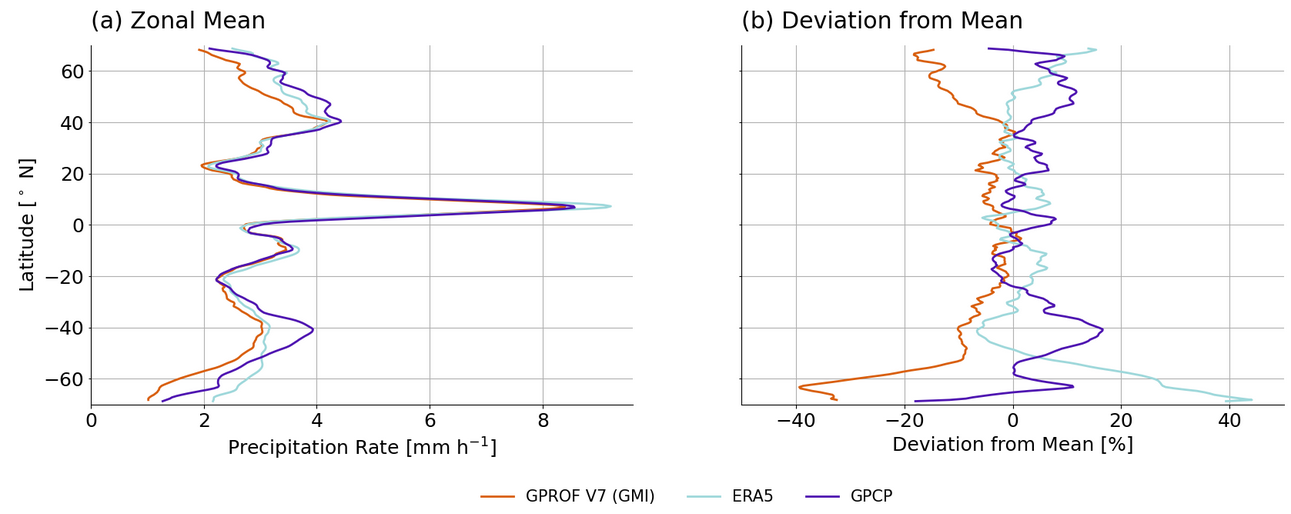
\includegraphics[width=37pc]{figures/figure01.png}}
  \caption{Zonal means of oceanic precipitation from GMI, the GPCP merged precipitation dataset, and the ERA5 reanalysis. Panel (a) shows absolute precipitation rates; Panel (b) shows relative deviations from the cross-dataset mean.}\label{fig:zonal_means}
\end{figure}

Recent neural-network precipitation retrievals \citep{pfreundschuh_gprof_2024}
have improved performance across many regimes and are being adopted
operationally. However, machine-learning retrievals approximate the conditional
expectation defined by their training data and thus reproduce biases present in
the reference observations. Training solely on DPR-based precipitation therefore
propagates the radar’s limited sensitivity to light and frozen precipitation
into the learned retrieval, regardless of retrieval technique used.

Here we aim to overcome the limitations of current DPR-based precipitation
estimates by using PMW observations to bridge the sensitivity gap between the
CPR and DPR precipitation estimates and thus achieve more complete
representation of precipitation across regimes. Specifically, we propose
GPROF-NN eXtended Precipitation Regime (XPR), a GMI-based retrieval that jointly
predicts precipitation estimates based on CPR- and DPR-based reference
precipitation rates. Since the CPR operates at a higher frequency, it is more
sensitive to small and frozen hydrometeors and can thus be expected to provide a
better representation of light and frozen precipitation. DPR, on the other hand,
misses light and frozen precipitation but provides reliable estimates of
moderate and heavy precipitation. The GPROF-NN XPR retrieval is trained to map
GMI PMW observations to both a light precipitation estimate based on CPR
reference data and an estimate of moderate to heavy precipitation based on DPR
reference data. As we will show here, an improved representation of
precipitation across regimes can be obtained by using the CPR-based
precipitation estimates to fill in missing light precipitation in the DPR-based
Estimates.

GPROF-NN XPR has been developed as an auxiliary retrieval to recover missing
oceanic precipitation in DPR-based reference data used by previous versions of
the GPROF and GPROF-NN \citep{pfreundschuh_gprof-nn_2022} retrievals. It is part
of the development of GPROF V08 -- the next operational version of the GPM PMW
retrievals -- and aims to address the systematic underestimation of high
latitude precipitation. The previous operational version of GPROF -- GPROF V07
-- used light precipitation estimates from the MiRS algorithm
\citep{boukabara_mirs_2011} to fill in missing precipitation in DPR estimates
but this was unsuccessful in fully addressing the underestimation. The filling
in of missing oceanic precipitation complements several other interventions
addressed to fix shortcomings in the DPR data used as a priori database and
training dataset such as the use of ground-based radar estimates over
snow-covered surface and the use of ERA5 precipitation over sea ice.

This manuscript describes the GPROF-NN XPR retrieval and validates its
precipitation estimates using in-situ measurements from shipborne distrometers
demonstrating its ability to improve the detection of light and frozen
precipitation and reduce  climatological biases. Additionally, we
provide a validation of the CPR- and DPR-based reference estimates against
independent measurements from ground-based precipitation radars.
Section~\ref{sec:methods} describes the retrieval implementation as well as the
data used to validate the retrievals. Section~\ref{sec:results} assesses and
validates the GPROF-NN XPR retrieval, validates the radar-based reference
estimates, and assesses the effect of the enhanced sensitivity of the GPROF-NN
XPR retrieval on the climatological precipitation distribution. Finally,
section~\ref{sec:summary} summarizes and discusses the main findings from this work.


\section{Methods and Data}
\label{sec:methods}

The GPROF-NN XPR retrieval algorithm is a machine-learning based precipitation
retrieval that is trained to simultaneously provide estimates of CPR-based and
DPR-based precipitation rates. The two estimates are subsequently fused to
provide a general precipitation estimate that better represents precipitation
across the full spectrum of intensities. Below we describe the retrieval
implementation together with the data sources used to validate the retrieval
itself as well as the two radar-based reference datasets.


\subsection{The GPROF-NN XPR Retrieval}

The GPROF-NN XPR retrieval is based on the GPROF-NN retrieval framework
introduced in \citep{pfreundschuh_gprof-nn_2022} and subsequently validated in
\citep{pfreundschuh_gprof_2024}. It uses the same neural-network architecture as
the upcoming version of GPROF-NN, which is currently under development and will
become the operational precipitation retrieval of the GPM constellation as GPROF
V08.

\subsubsection*{Neural Network Model}

The GPROF-NN XPR retrieval employs a U-Net–type encoder–decoder architecture
composed of EfficientNet-V2–style inverted bottleneck convolutional blocks
\citep{tan2021efficientnetv2}. Following the normalization and activation design
adopted in ConvNeXt \citep{liu2022convnet}, each convolutional block uses Layer
Normalization \citep{ba2016layer} and GELU activation functions
\citep{hendrycks2016gaussian}. The network input consists of GMI brightness
temperatures together with the corresponding earth-incidence angles (EIA) for
all channels and a set of ancillary variables. These ancillary data describe
both surface conditions (land fraction, elevation, mountain classification,
leaf-area index, ice fraction, and snow depth) and the meteorological
environment (2-m temperature, 10-m wind speed, orographic wind, and total column
water vapor).

The model produces two precipitation estimates: one trained on CPR-based
reference precipitation and one trained on DPR-based reference precipitation.
Both estimates are derived from a shared latent representation using separate
multilayer perceptron output heads. Each head predicts 32 quantiles of the
conditional precipitation distribution, which are learned using quantile
regression \citep{pfreundschuh_neural_2018}. The expectation is that the
CPR-based reference data will miss heavy rain where CPR is attenuated while the
DPR-based reference will miss light precipitation below the detection threshold
of those radars.

\begin{figure}[h]
 \centerline{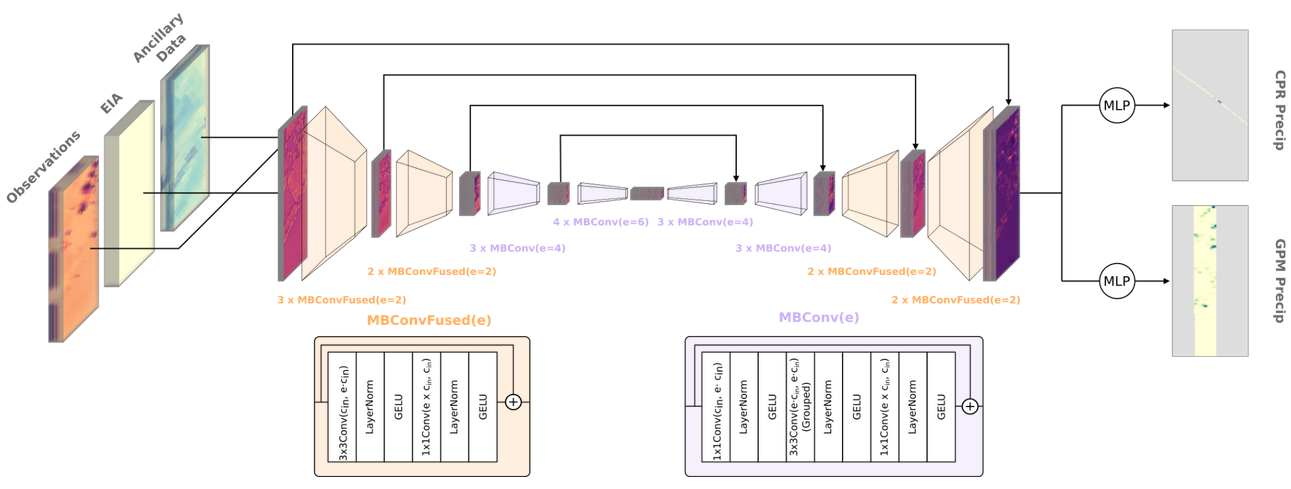
\includegraphics[width=37pc]{figures/figure02.png}}
 \caption{
   Illustration of the U-Net neural network used by GPROF-NN XPR. The network
   employs MobileNet convolutional blocks (MBConv) within an encoder–decoder
   architecture. Input features consist of image patches of GMI brightness
   temperatures, corresponding earth-incidence angles (EIA), and ancillary
   variables. These inputs are mapped to a shared latent representation from which
   two precipitation estimates are derived through separate output heads: a
   CPR-based light precipitation estimate and a DPR-constrained
   moderate-to-heavy precipitation estimate.
 }\label{fig:neural_network}
\end{figure}

\subsubsection*{Training Data and Training}

The training dataset for the GPROF-NN XPR retrieval is constructed from two
independent sets of collocations between GMI observations and reference
precipitation estimates from the CPR and DPR sensors.

For the GMI--CPR dataset, precipitation estimates are derived by combining
information from the 2C-Precip-Column \citep{haynes_2009}, 2C-Rain-Profile
\citep{lebsock_2011}, and 2C-Snow-Profile \citep{wood_2014} products.
Precipitation rates are assigned according to the precipitation classification
in 2C-Precip-Column: pixels flagged as non-precipitating are assigned zero
precipitation; pixels classified as certain rain are assigned the rate from
2C-Rain-Profile; pixels classified as certain snow are assigned the rate from
2C-SnowProfile. Pixels that do not meet any of these conditions or are assigned
a retrieval confidence less than three are treated as missing and excluded from
training. The dataset includes all GMI-CPR collocations from 2014–2017 with a maximum
temporal separation of 15 min between the GMI and CloudSat observations.
Collocations from January–October 2018 are used for validation, and those from
October 2018–October 2019 are reserved for testing.

For the GMI–DPR dataset, precipitation rates are taken from the GPM 2BCMB \citep{grecu2016gpm}
combined radar–radiometer product. Because GMI and DPR observe from the same
platform, these collocations are substantially more numerous than the
GMI–CloudSat matchups. During training, the GMI–CloudSat samples are therefore
oversampled such that, on average, every second training sample originates from
the GMI–CloudSat dataset, ensuring comparable representation of both reference
regimes. The training is performed across 120 epochs using a cosine-annealing
learning-rate schedule with an initial learning rate of 0.0005 and warm restarts
after 20 and 60 epochs.

\subsubsection*{Fused Precipitation Estimates}

The GPROF-NN XPR retrieval produces CPR-based and a DPR-based precipitation
estimate for each GMI pixel. To provide a single precipitation estimate that
properly describes precipitation across precipitation regimes, the two estimates
must be combined. The fused estimate relies on the CPR-based estimate when the
DPR-based retrieval indicates no precipitation (reflectivities below the DPR
threshold) and transitions to the DPR-based estimate as intensity increases
(reflectivities likely attenuated in CPR). A simple linear transition, however,
was found to introduce a notable artifact in the distribution of the fused
precipitation rates. Instead, a zero-centered Gaussian weighting function was
applied to obtain a smooth precipitation-rate distribution. The Gaussian has a
full width at half maximum of 0.45 $mm h^{-1}$, with the resulting weighting
function as well as the distribution of test-data precipitation rates shown in
Fig.~\ref{fig:fused_distributions}.

The distribution of the fused precipitation estimates follows that of the
CPR-based estimates at low precipitation rates and transitions to follow the
distribution of the DPR-based precipitation rates for moderate to high
precipitation. The distribution of the GPROF-NN CPR precipitation estimates
exhibits several irregularities and is less smooth than that of the GPROF-NN DPR
estimates. We suspect that this may be related to the bimodal distribution of
the 2C-Rain-Profile estimates that was noted already in Lebsock (2011). While
the bulges in the PDF of GPROF-NN CPR precipitation estimates do not match the
exact peaks of the distribution in Fig. 7 in Lebsock (2011), they may be shifted
in the retrieved distributions due to the increased resolution of the GMI-based
GPROF-NN retrievals.

\begin{figure}[h]
 \centerline{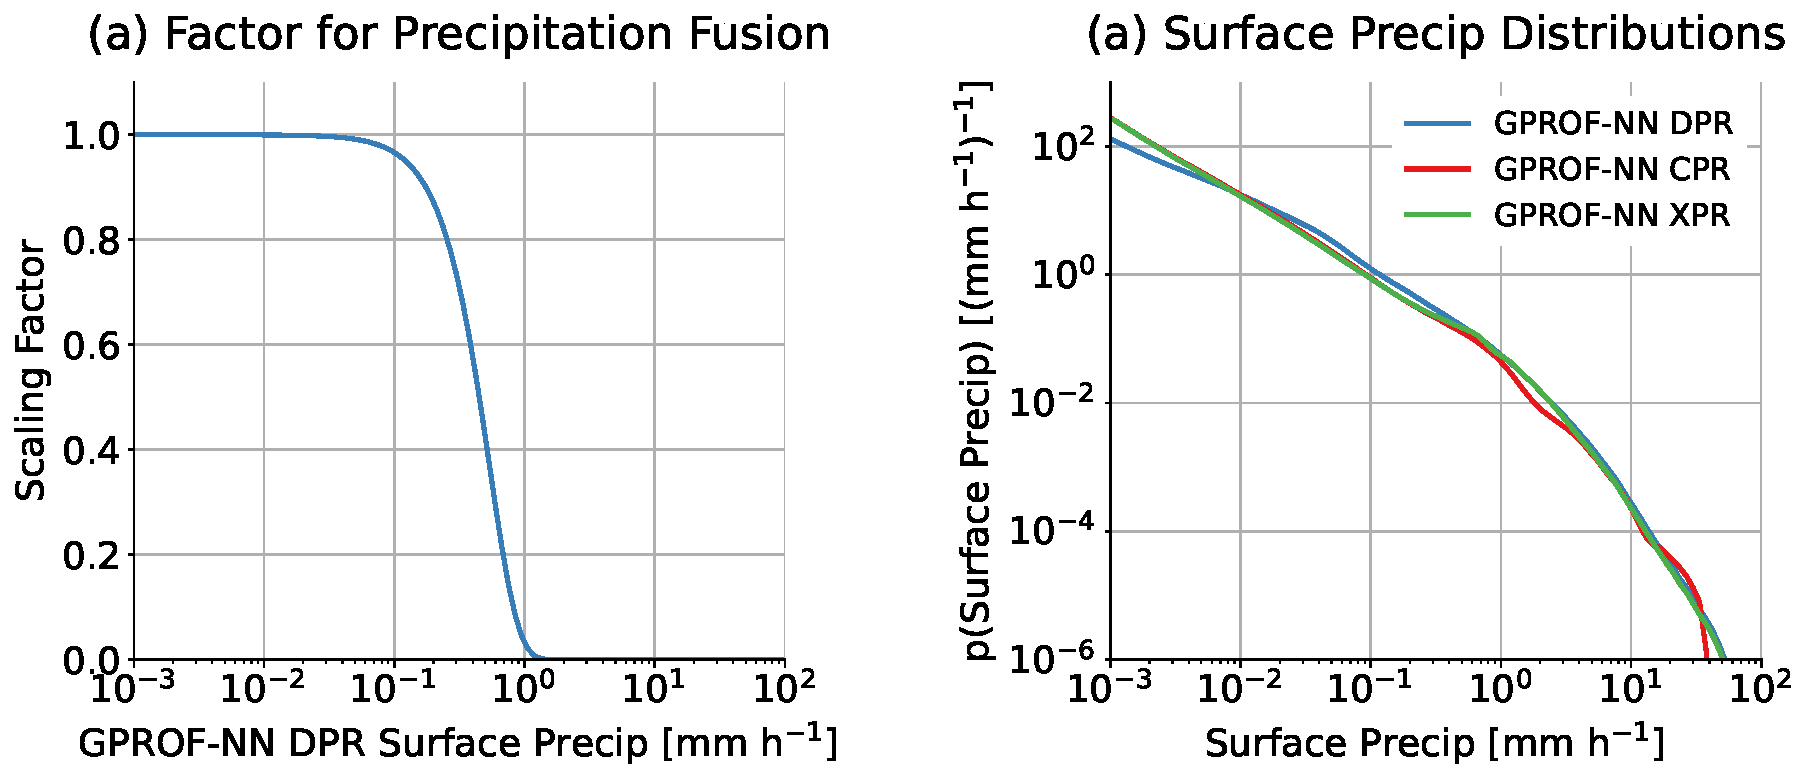
\includegraphics[width=37pc]{figures/figure03.pdf}}
 \caption{
Scaling factors used to fuse CPR- and DPR-based precipitation estimates (a) and
resulting precipitation rate distributions (b).
 }\label{fig:fused_distributions}
\end{figure}

\subsection{Validation Data}

We validate both the GPROF-NN XPR retrieval and the underlying CPR- and
DPR-based precipitation estimates using independent observations. The GMI-based
GPROF-NN XPR estimates are validated against in situ measurements from shipborne
disdrometers, which provide the most direct reference data available for oceanic
precipitation. Owing to the much narrower swaths of the DPR and CPR, there are
not enough overpasses to meaningfully evaluate the radar-based reference
estimates with the shipborne measurements. Instead, their consistency is
assessed using overpasses along the U.S. East Coast, where the satellite
estimates are compared with coincident observations from ground-based weather
radars.

\subsubsection*{OceanRAIN Ship-Based Distrometer Measurements}

\begin{figure}[h]
 \centerline{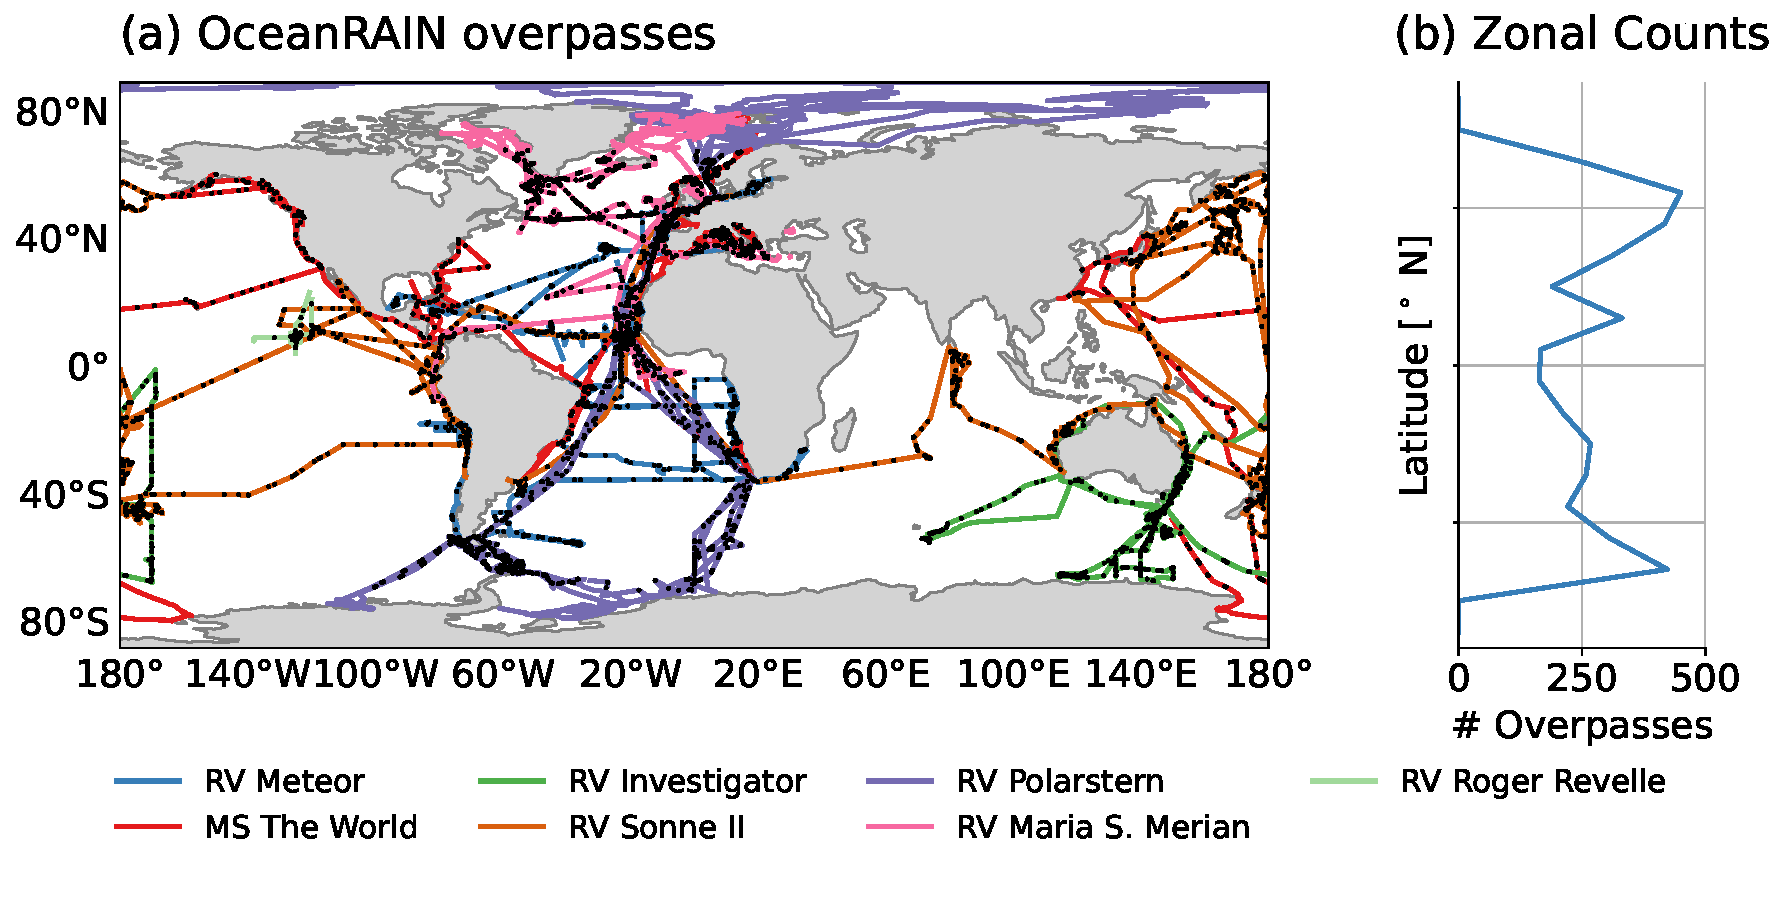
\includegraphics[width=37pc]{figures/figure04.pdf}}
 \caption{
OceanRAIN ship tracks and corresponding GMI overpasses. Colored lines indicate
the trajectories of OceanRAIN vessels during the GMI observation period, and
black dots denote the collocated satellite overpasses used for validation of the
GPROF-NN XPR retrieval.
 }\label{fig:ocean_rain_collocs}
\end{figure}

The OceanRAIN dataset \citep{klepp2018oceanrain} provides shipborne disdrometer
measurements of precipitation rates over the ocean. For validation of the
GPROF-NN XPR retrieval, we identify GMI overpasses of the ship locations from
March 2014, the start of GMI observations, through September 2018, prior to the
period used for GPM-DPR training collocations. Because this interval overlaps
with the GMI–CloudSat training dataset, any coincident matchups are excluded
from the evaluation.

Figure~\ref{fig:ocean_rain_collocs} shows the ship tracks associated with the OceanRAIN campaigns together
with the corresponding GMI overpasses. To account for the spatial scale mismatch
between satellite footprints and point measurements, the satellite estimates are
compared with 30-min rolling averages of the disdrometer precipitation rates.
The matched retrieved precipitation is computed by calculating the pixel closest to
the ship position for each minute in the averaging window and calculating the corresponding
average.

To eliminate the impact of errors in the validation data, we calculate a relative error using

\begin{align}
  \text{err} = \frac{|p_\text{retrieved} - p_\text{reference}|}{max(0.5, 0.5 \cdot |p_\text{retrieved} + p_\text{reference}|)}
\end{align}

The error is calculated for the GPROF-NN DPR retrieval as well as the
corresponding GPROF V07 and ERA5 precipitation estimates. Samples where the
minimum relative error across these three datasets exceeds 1.8 are discarded. In
total, 26 samples from the 3436 collocations with valid precipitation estimates
fail to meet this quality criterion. The removed overpasses correspond to
precipitation events missed by the distrometer as well as cases where the
distrometer indicates very high precipitation rates not seen in the satellite or
ERA5 data. The exclusion of these events does not impact the qualitative results
of the validation.

\subsubsection*{Ground-Based Precipitation Radar Estimates}

\begin{figure}[h]
 \centerline{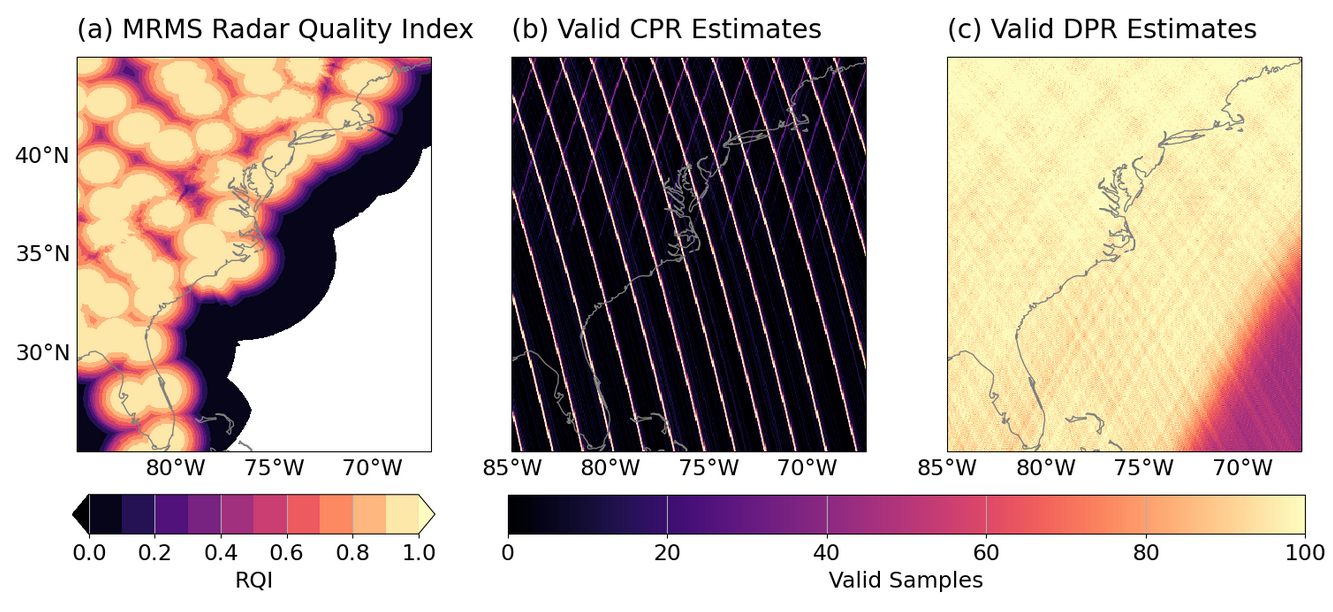
\includegraphics[width=37pc]{figures/figure05.png}}
 \caption{
Summary statistics the validation data derived from NOAA’s Multi-Radar
Multi-Sensor data. Panel (a) shows the radar-quality index quantifying the
quality of the radar measurements. Panel (b) and (c ) show the mean
precipitation and precipitation occurrence, respectively.
 }\label{fig:radar_overpasses}
\end{figure}

To provide additional context for the evaluation of the GPROF-NN XPR retrieval,
we assess the CPR and DPR reference precipitation estimates using independent
observations from NOAA’s Multi-Radar Multi-Sensor (MRMS) product along the U.S.
East Coast. For the CPR-based estimates, all available overpasses from June 2015
through the end of the CloudSat mission are included. Owing to the wider swath
of the DPR, overpasses from the year 2022 alone provide sufficient sampling for
a robust comparison.

Because this study focuses on oceanic precipitation, only satellite pixels
located over the ocean are retained. Since the chance for beam overshoot
increases with distance from the shore, only MRMS pixels with a radar quality
index (RQI) exceeding 0.9 are retained, limiting the distance to the closest
radar to about 100 km. As RQI fields are unavailable for some earlier MRMS
periods, the mean RQI field from 2022 is used to screen the matched
observations. Following Pfreundschuh (2026), the MRMS precipitation fields are
aggregated to a $0.36^\circ \times 0.36^\circ$ grid and collocated with the CloudSat and
DPR estimates using nearest-neighbor interpolation. Panel (a) of Fig. 5 presents
the mean radar quality index (RQI) used to filter valid match-ups. Even with a
minimum RQI threshold of 0.9, the NEXRAD network provides coverage across most
of the U.S. East Coast. Panels (b) and (c) display the total number of valid
precipitation retrievals extracted within the validation domain before the RQI
mask is applied. Valid CloudSat retrievals are largely limited to ascending
overpasses due to its restriction to daytime-only operation during the
validation period. A smaller number of descending overpasses are available over
the northern portion of the domain during summer. In contrast, the substantially
wider swath of the DPR results in far more frequent observations that are
distributed more uniformly across the domain.


\section{Results}
\label{sec:results}

Below we present the three principal results from this work: Firstly, we assess
the accuracy of the GPROF-NN XPR retrieval by comparing it to GPM CMB and
CloudSat estimates from independent testing periods and a case study from the
validation period. Following this, we validate the fused GPROF-NN XPR retrieval
as well as CPR- and DPR-based precipitation estimates against independent
in-situ precipitation estimates. Finally, we compare global retrieval statistics
to existing datasets to assess the impact of the expanded reference data on the
GPROF-NN XPR retrievals.

\subsection*{Retrieval Accuracy}

Figure~\ref{fig:test_results} shows scatter plots of reference and retrieved
precipitation rates for the CPR- and DPR-based outputs of the GPROF-NN XPR
retrieval. The retrieval reproduces the DPR-based estimates well, achieving low
bias and mean-squared error and high linear correlation. The accuracy of the
CPR-based estimates is substantially lower: MSE and correlation coefficient
indicate lower accuracy that is also reflected in the increased spread of the
retrieved values. In part, this can be explained by the higher resolution of the
CPR-based precipitation estimates. Both training and testing data uses CPR
estimates at the native resolution (1.6 km), whereas the DPR-based estimates are
downsampled to the GMI resolution, which is how they are traditionally treated
in the GPROF framework. The different approach for the CPR-based estimates was
chosen due to the difficulties of assigning a unique resolution to the GMI
observations and downsampling the one-dimensional CPR data to the
two-dimensional GMI footprints.

The CPR-based precipitation estimates show fair agreement with the reference
values from 0.1 to 3--4 mm/h but struggle to reproduce precipitation estimates
exceeding that. However, since CloudSat estimates have to be considered very
uncertain in this range, it is possible that this is – at least in part – due to
errors in the CPR-based reference data. Additionally, there is a notable bias in
the CPR-based precipitation estimates of about 13\% which is caused by the
underestimation of the higher rain rates. Given that precipitation rates
exceeding 3-4 mm/h account for more than 10 \% of the total precipitation in the
test data, the bias may be caused by statistical fluctuations and the smaller
number of testing samples compared to the DPR-based estimates. Furthermore,
since CloudSat left the A-train in 2018, the precipitation estimates from the
test data were derived in a different orbital configuration, which can further
affect bulk precipitation statistics and thus produce biases in the test
results.

\begin{figure}[h]
 \centerline{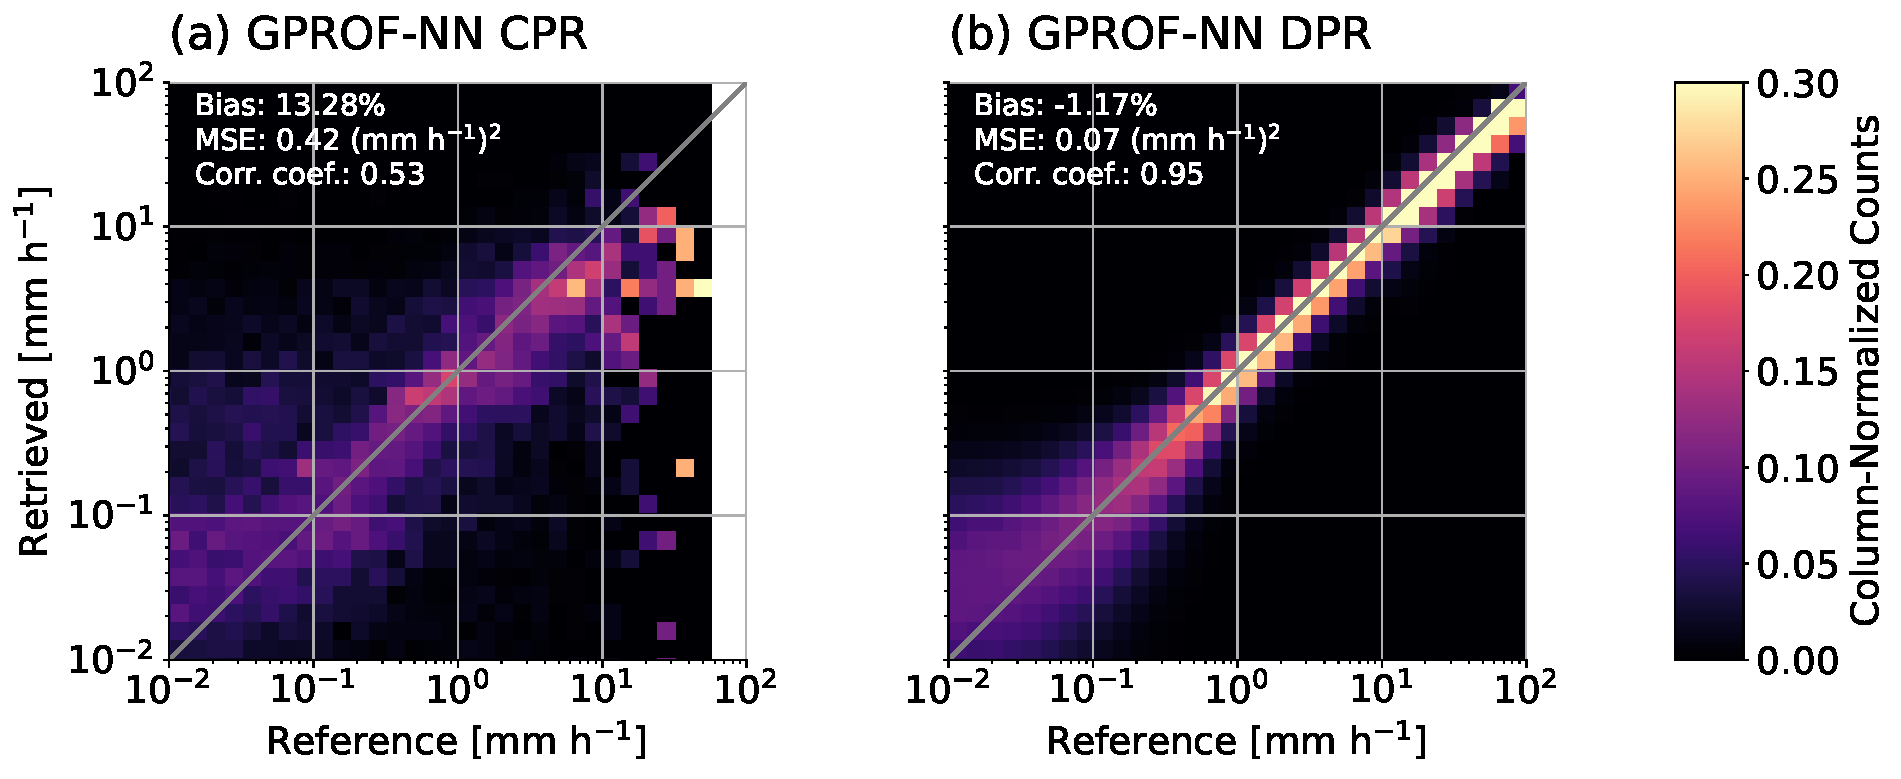
\includegraphics[width=37pc]{figures/figure06.pdf}}
 \caption{
   Scatter plots of reference and retrieved precipitation for the (a) CPR-based
   and (b) the DPR-based precipitation estimates.
 }\label{fig:test_results}
\end{figure}


\subsection*{Case Study}

Figure~\ref{fig:case_study} illustrates an example of the DPR- and CPR-based
precipitation estimates together with the resulting fused estimate. The case
study displays a GMI overpass of a Southern Hemisphere mid-latitude cyclone in
June 2018. A comparison of the CPR-based, DPR-based, and fused XPR precipitation
fields highlights substantial structural differences among the three products.
Although the CPR- and DPR-based estimates are generated using the same model,
they exhibit marked discrepancies. The CPR-based retrieval produces higher
precipitation intensities and a broader spatial extent of the cyclone’s
precipitation field. The fused XPR product moderates the elevated precipitation
rates evident in the CPR-based retrieval while largely preserving its enhanced
spatial coverage.

Comparison with the reference data along the CloudSat swath shows that the
GPROF-NN XPR retrieval successfully captures the shallow precipitation occurring
between 200 and 250 km along the CloudSat track that is missed by both the DPR
reference estimates and the GPROF-NN DPR retrievals. Generally, the GPROF-NN XPR
results capture the main precipitation features but do not reproduce the
small-scale variability present in the radar-based reference estimates. This
discrepancy is expected because PMW observations have coarser spatial resolution
and sampling than the radar measurements. A around 50 km and 750 km along the
swath, the GPROF-NN XPR retrieval indicates precipitation while the CPR-based
estimates suggest little or no precipitation. However, the CPR radar still
detects reflectivities extending down to the surface in these regions,
suggesting that precipitation likely reaches the surface but may be
overestimated by the PMW retrieval.


\begin{figure}[h]
 \centerline{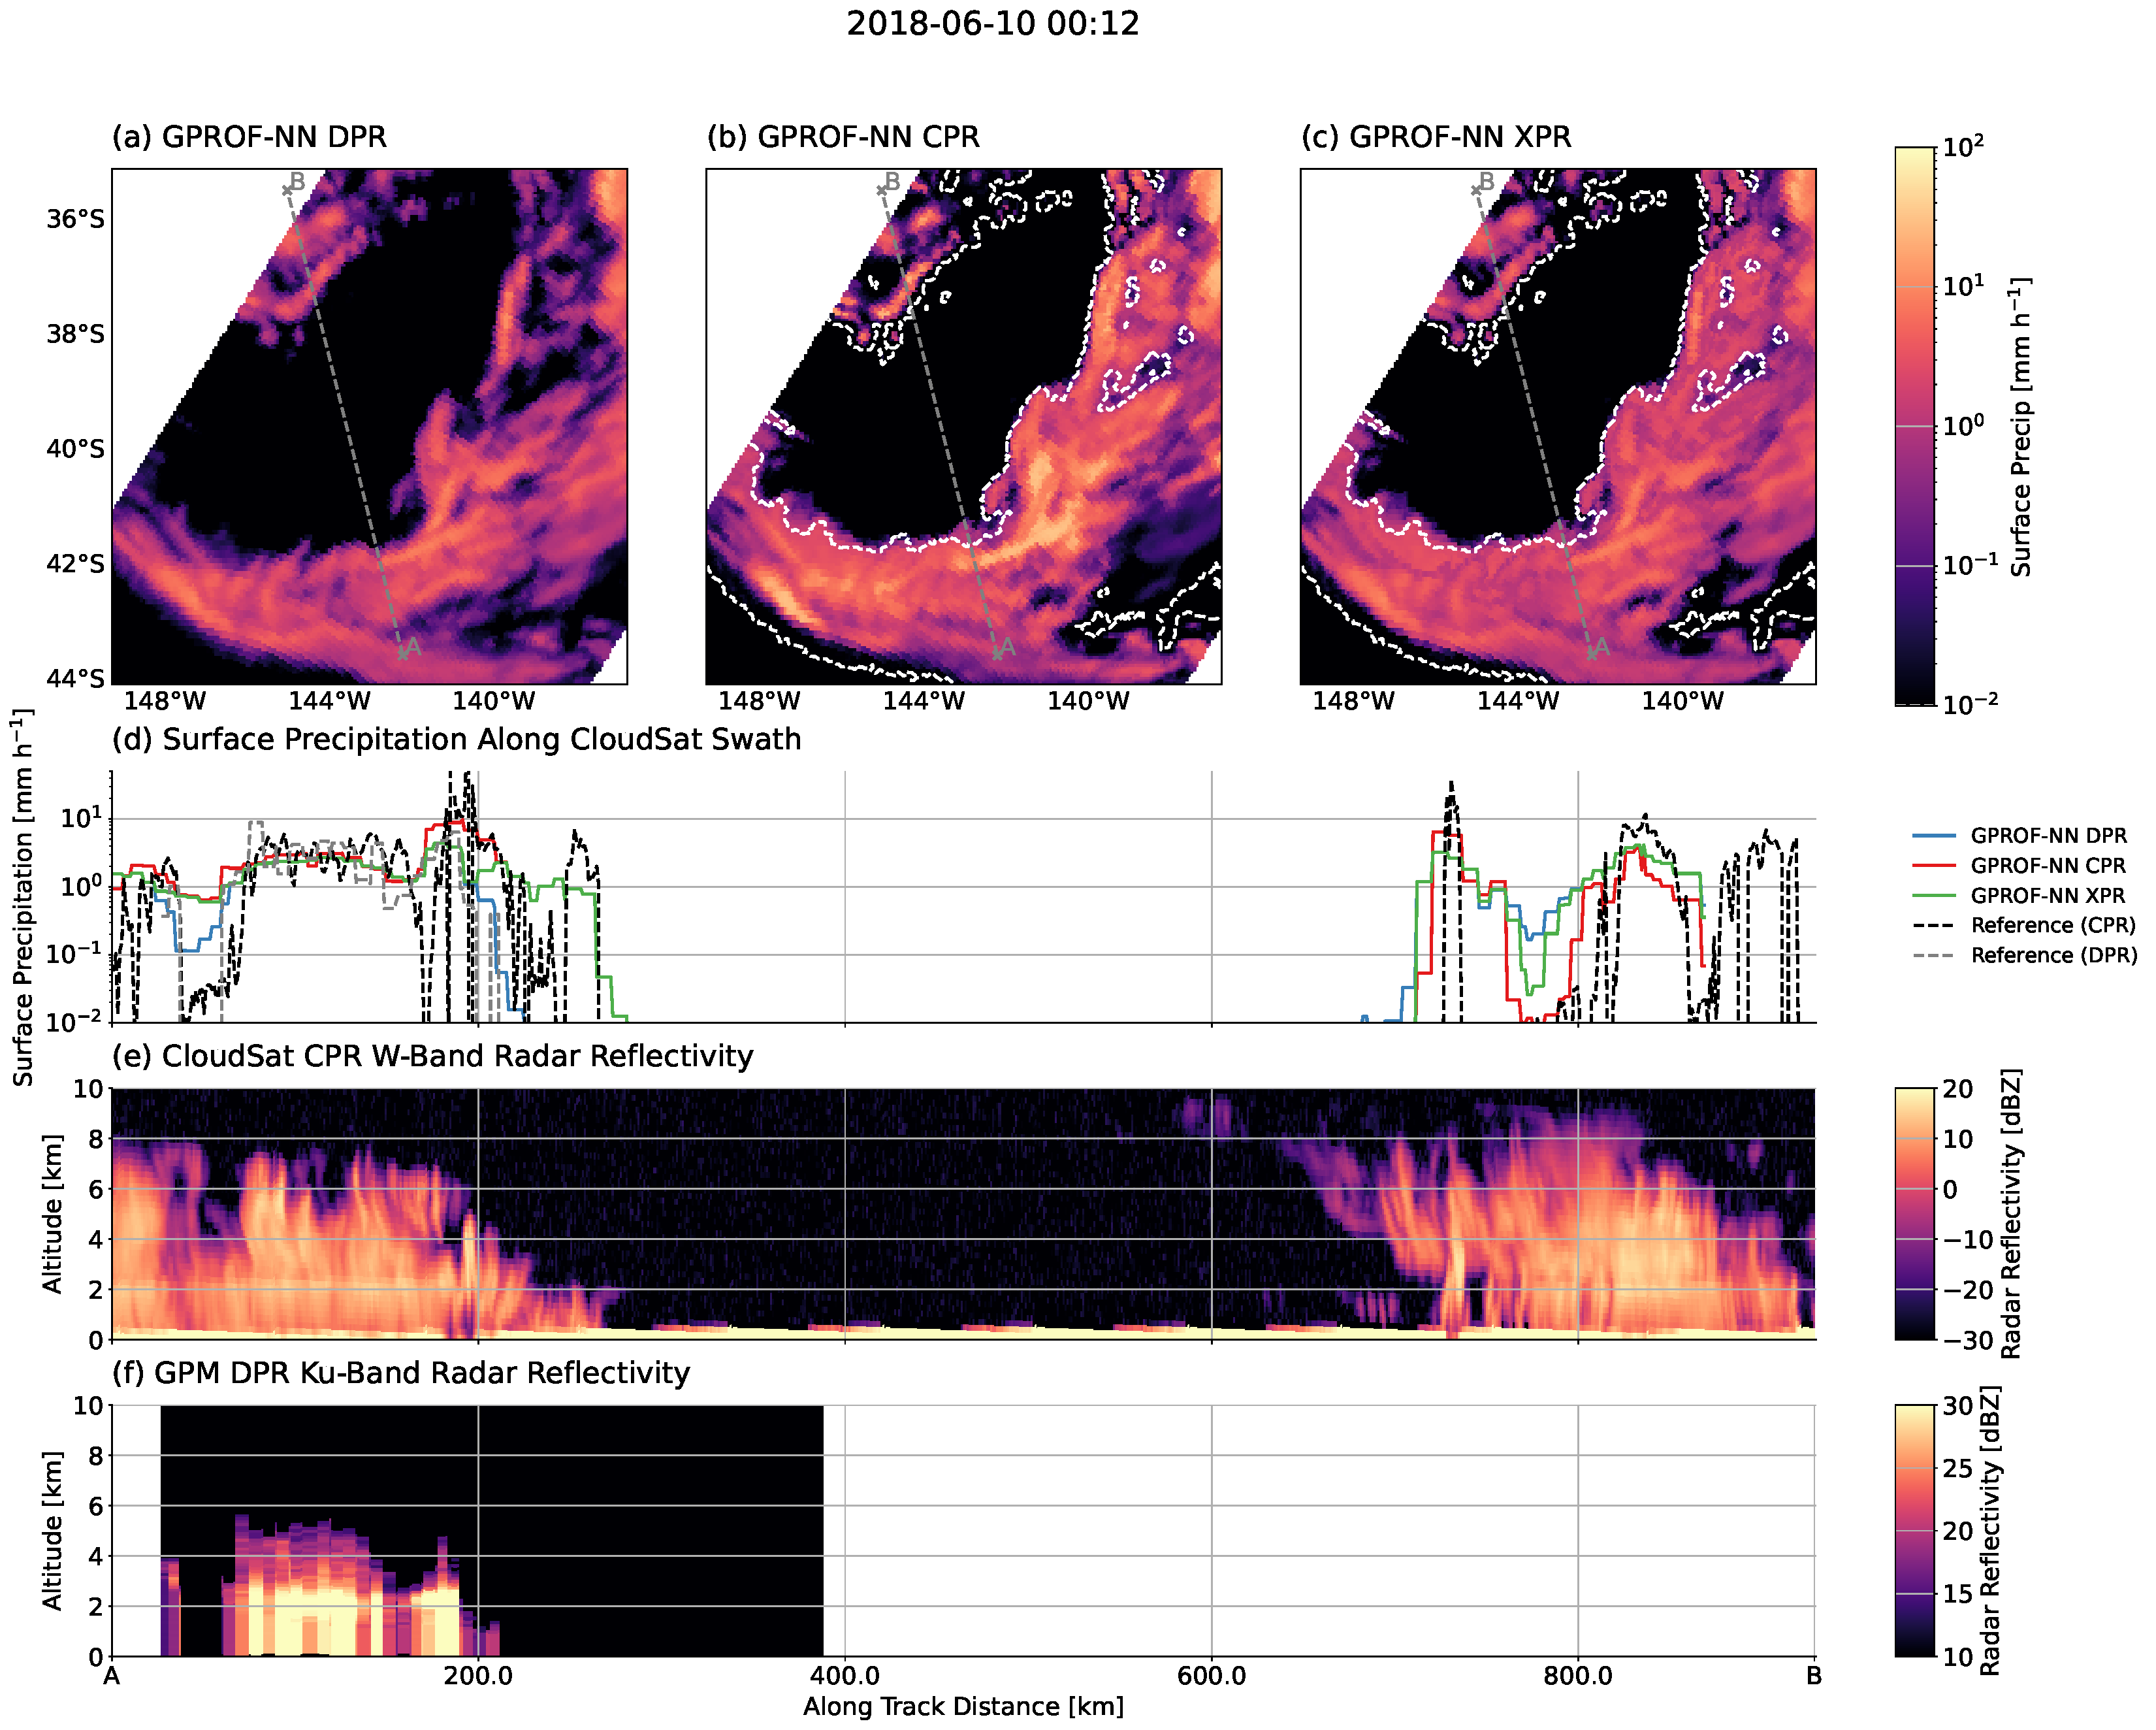
\includegraphics[width=37pc]{figures/figure07.pdf}}
 \caption{
   Coincident observations of a mid-latitude cyclone by the GPM and CloudSat
   satellites. The first row of panels displays GMI-based PMW retrievals trained on
   GPM DPR precipitation (a), on CloudSat CPR precipitation (b), and the fused
   precipitation field combining the DPR- and CPR-based estimates (c ). Panels (d),
   (e), and (f) show the retrieved precipitation and the corresponding CloudSat and
   GPM radar reflectivities along the CloudSat swath.
 }\label{fig:case_study}
\end{figure}

\subsection{Validation}

The results presented above demonstrate that the GPROF-NN XPR retrieval is able
to reproduce both CPR- and DPR-based precipitation estimates accurately
considering the differences in resolution and information content of the PMW
observations as well as the sensitivity ranges of the two reference datasets.
However, since neither reference dataset accurately captures precipitation
accurately across the full spectrum of precipitation intensities, it is
essential to evaluate the GPROF-NN XPR retrieval against independent
precipitation measurements to ensure it actually improves the representation of
precipitation cipitation. Below we validate both the GPROF-NN XPR retrieval as
well as the reference datasets themselves against independent precipitation
measurements.

\subsection{OceanRAIN}

The GPROF-NN XPR precipitation estimates are evaluated using 3,589 OceanRAIN
overpasses that passed quality control and yielded valid precipitation estimates
from GPROF V07, ERA5, and GPROF-NN XPR. To provide a more granular assessment,
we stratify the analysis into three subsets: (1) all overpasses, (2)
high-latitude cases poleward of 45°, and (3) scenes with a high likelihood of
mixed or frozen precipitation. The latter classification uses the
parameterization of \citet{sims2015parametrization} with ERA5-derived wet-bulb
temperatures. Overpasses with a conditional probability of solid precipitation
exceeding 50\% are categorized as likely mixed or frozen precipitation events.

\subsubsection*{Precipitation Detection}

\begin{figure}[h]
 \centerline{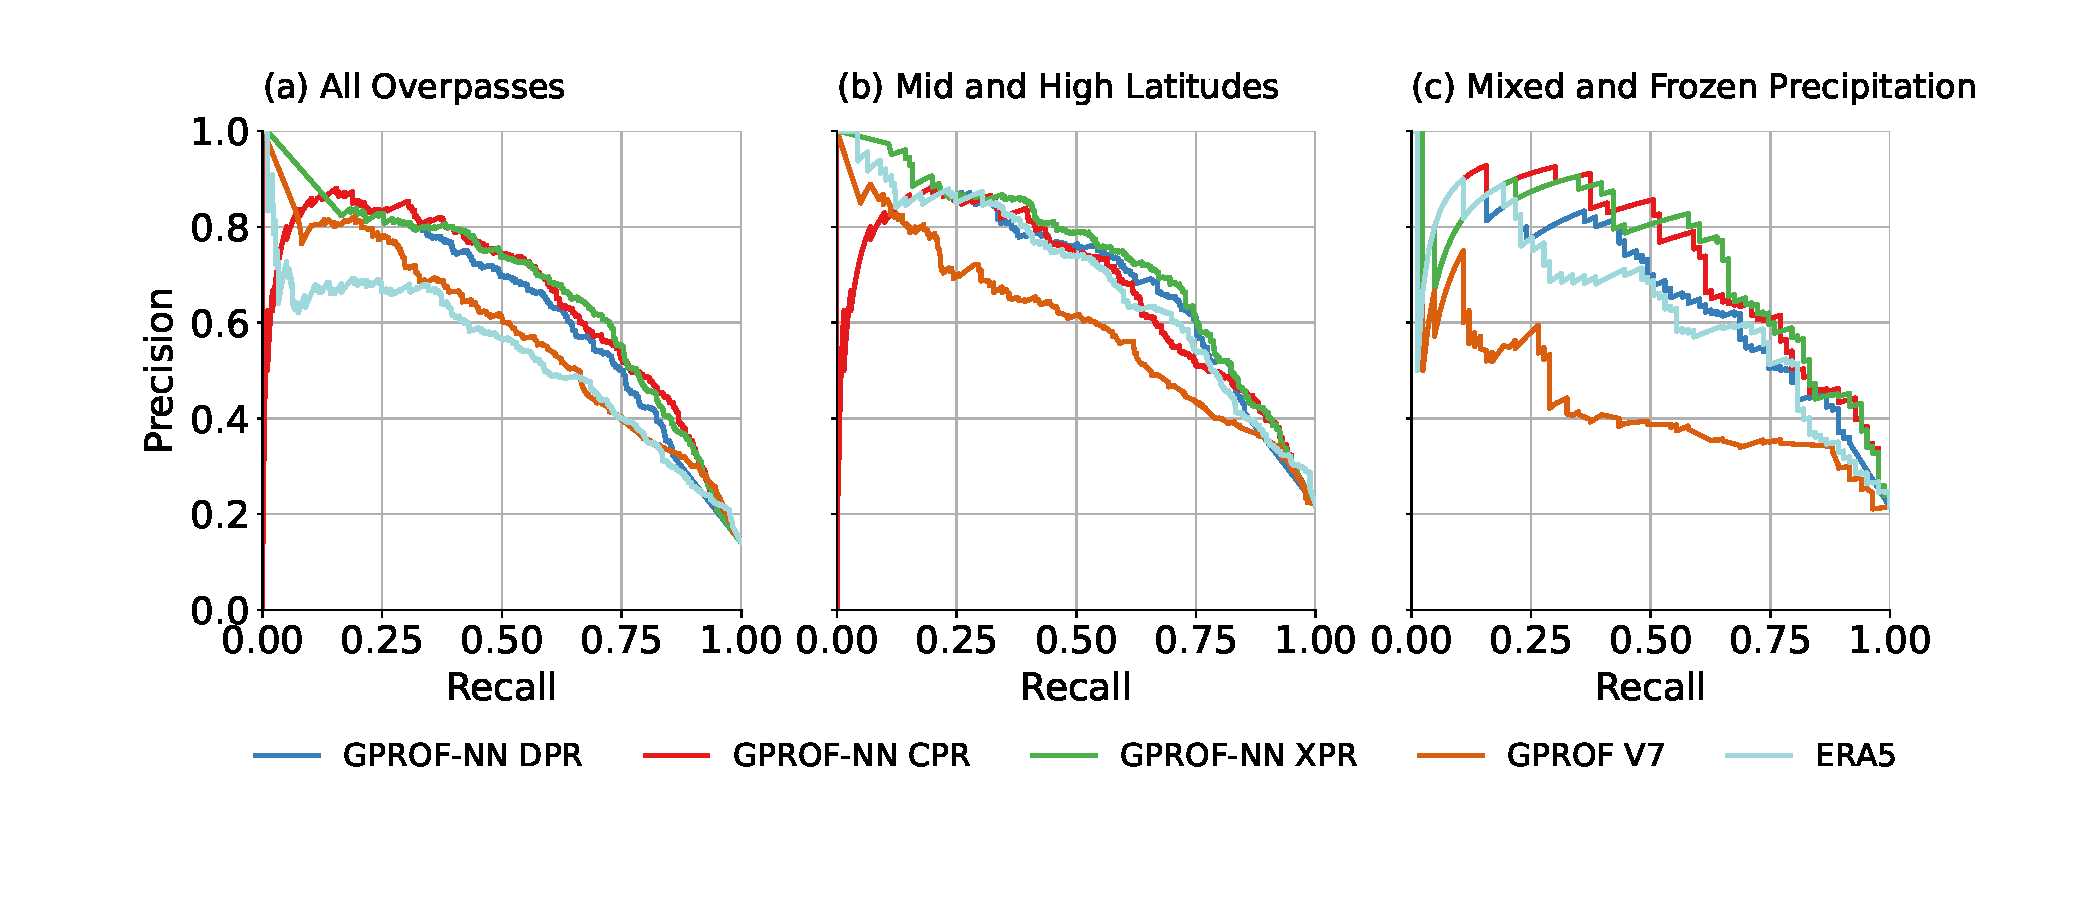
\includegraphics[width=37pc]{figures/figure08.pdf}}
 \caption{
    Precipitation-detection skill evaluated against ship-borne distrometer
    measurements. Each panel shows precision–recall curves for the GPROF-NN XPR
    retrieval outputs based on CPR estimates (GPROF-NN CPR), the DPR-based
    precipitation estimates (GPROF-NN DPR), the fused estimates (GPROF-NN XPR) and
    the GPROF V07 and ERA5 baselines. c Panels (a) – (c ) show precipitation
    estimates for all overpasses, overpasses for latitudes poleward of 45°, and for
    mixed and frozen precipitation, respectively.
 }\label{fig:ocean_rain_detection}
\end{figure}

We first assess the detection capability of the three GPROF-NN retrievals as
well as GPROF V07 and ERA5 baselines using precision-recall curves. The
precision recall curves display the trade off between precision, i.e., the
probability of a detection being correct, and the recall, i.e., the fraction of
total precipitation events detected, as the probability threshold used to decide
whether a pixel raining or not is varied. The more skillful the detection, the
closer the curve gets to a precision and recall value of one. All GPROF
retrievals provide a probability of precipitation representing the estimated
probability of the corresponding pixel containing precipitation. Since ERA5
doesn’t provide a dedicated probability field for precipitation occurrence, we
use the precipitation rate as detection criterion. An overpass is defined to be
precipitating when the half-hour average distrometer precipitation exceeds 0.01
mm/h.

Figure~\ref{fig:ocean_rain_detection} displays the precipitation detection
accuracy for all overpasses, overpasses at high latitudes, and mixed and frozen
precipitation. Considering all overpasses, the CloudSat-based light
precipitation and the fused GPROF-NN XPR results yield the highest detection
accuracy. This is consistent with the CloudSat-based precipitation estimates
providing higher sensitivity to light precipitation that is missed by the GPM
DPR reference data. The retrieval based solely on GPM DPR data has slightly
lower detection skill but remains clearly more sensitive than the GPROF V7 and
ERA5 baselines.

Somewhat surprisingly, the detection accuracy of the DPR-based estimates exceeds
that of the CPR-based estimates at mid and high latitudes. This seems to
indicate that the CPR-based GPROF-NN estimates miss certain precipitation events
that are detected by the DPR-based estimates but it is not immediately clear for
which precipitation processes this would occur. The GPROF-NN XPR achieves the
highest precipitation detection skill exceeding that of both the CPR- and the
DPR-based retrievals.

Although the results for mixed and frozen precipitation are overall noisier, the
CPR-based and fused precipitation estimates clearly achieve the best detection
accuracy. The DPR-based retrieval performs worse and is closely followed by
ERA5. The GPROF V7 retrieval performs substantially worse with the best
precision and recall values being about half of the GPROF-NN XPR retrieval.

Table~\ref{tab:detection_metrics} evaluates the detection skill of all
retrievals that provide a probability of precipitation using a probability
threshold of 0.5. This evaluation confirms that the GPROF-NN XPR retrieval
yields the best detection skill across all precipitation regimes. In particular,
the GPROF-NN XPR retrieval improves the detection skill compared to GPROF-NN DPR
by 48 \%, 26 \%, and 42 \% for all overpasses, mid and high latitudes
overpasses, and frozen precipitation, respectively.


\begin{table}[t]
\centering
\caption{Precipitation detection metrics (POD, FAR, CSI) for different retrieval methods evaluated against shipborne distrometer measurements across precipitation regimes.}
\label{tab:detection_metrics}
\begin{tabular}{lccccccccc}
\toprule
& \multicolumn{3}{c}{All Overpasses} 
& \multicolumn{3}{c}{Mid and High Latitudes} 
& \multicolumn{3}{c}{Frozen Precipitation} \\
\cmidrule(lr){2-4} \cmidrule(lr){5-7} \cmidrule(lr){8-10}
Method 
& POD & FAR & CSI 
& POD & FAR & CSI 
& POD & FAR & CSI \\
\midrule
GPROF V07    & 0.37 & 0.31 & 0.32 & 0.29 & 0.28 & 0.26 & 0.11 & 0.25 & 0.10 \\
GPROF-NN DPR & 0.85 & 0.65 & 0.33 & 0.85 & 0.56 & 0.41 & 0.90 & 0.63 & 0.36 \\
GPROF-NN CPR & 0.44 & 0.23 & 0.39 & 0.45 & 0.23 & 0.40 & 0.66 & 0.35 & 0.49 \\
GPROF-NN XPR & 0.67 & 0.35 & 0.49 & 0.65 & 0.28 & 0.52 & 0.71 & 0.36 & 0.51 \\
\bottomrule
\end{tabular}
\end{table}

\subsubsection*{Precipitation Estimation}

Figure~\ref{fig:ocean_rain_scatter} assesses the quantitative precipitation
estimates of the GPROF-NN retrievals with respect to the OceanRAIN reference.
The GPROF-NN DPR retrieval achieves higher correlation with the OceanRAIN
measurements than the CPR-based estimates. The CPR-based estimates exhibit
higher spread at both low- and high-precipitation rates. To assess the impact of
the precipitation-rate fusion, panel (c) displays the relative change in the
symmetric mean percentage error (SMAPE) resulting from the combining of the DPR-
and CPR-based estimates compared to the DPR baseline. While the merging
decreases the SMAPE for a significant number of samples close to the diagonal,
the are a notable amount of samples for which the SMAPE is increased. Most of
these correspond to the merging leading to an overestimation of the
precipitation. Since the coloring indicates the increase in the relative error,
the largest increases in error occur at small reference precipitation rates as
the relative error is more sensitive in these regimes. For red samples below the
diagonal, the merging with the CPR estimates erroneously reduces the final
precipitation rate.

\begin{figure}[h]
 \centerline{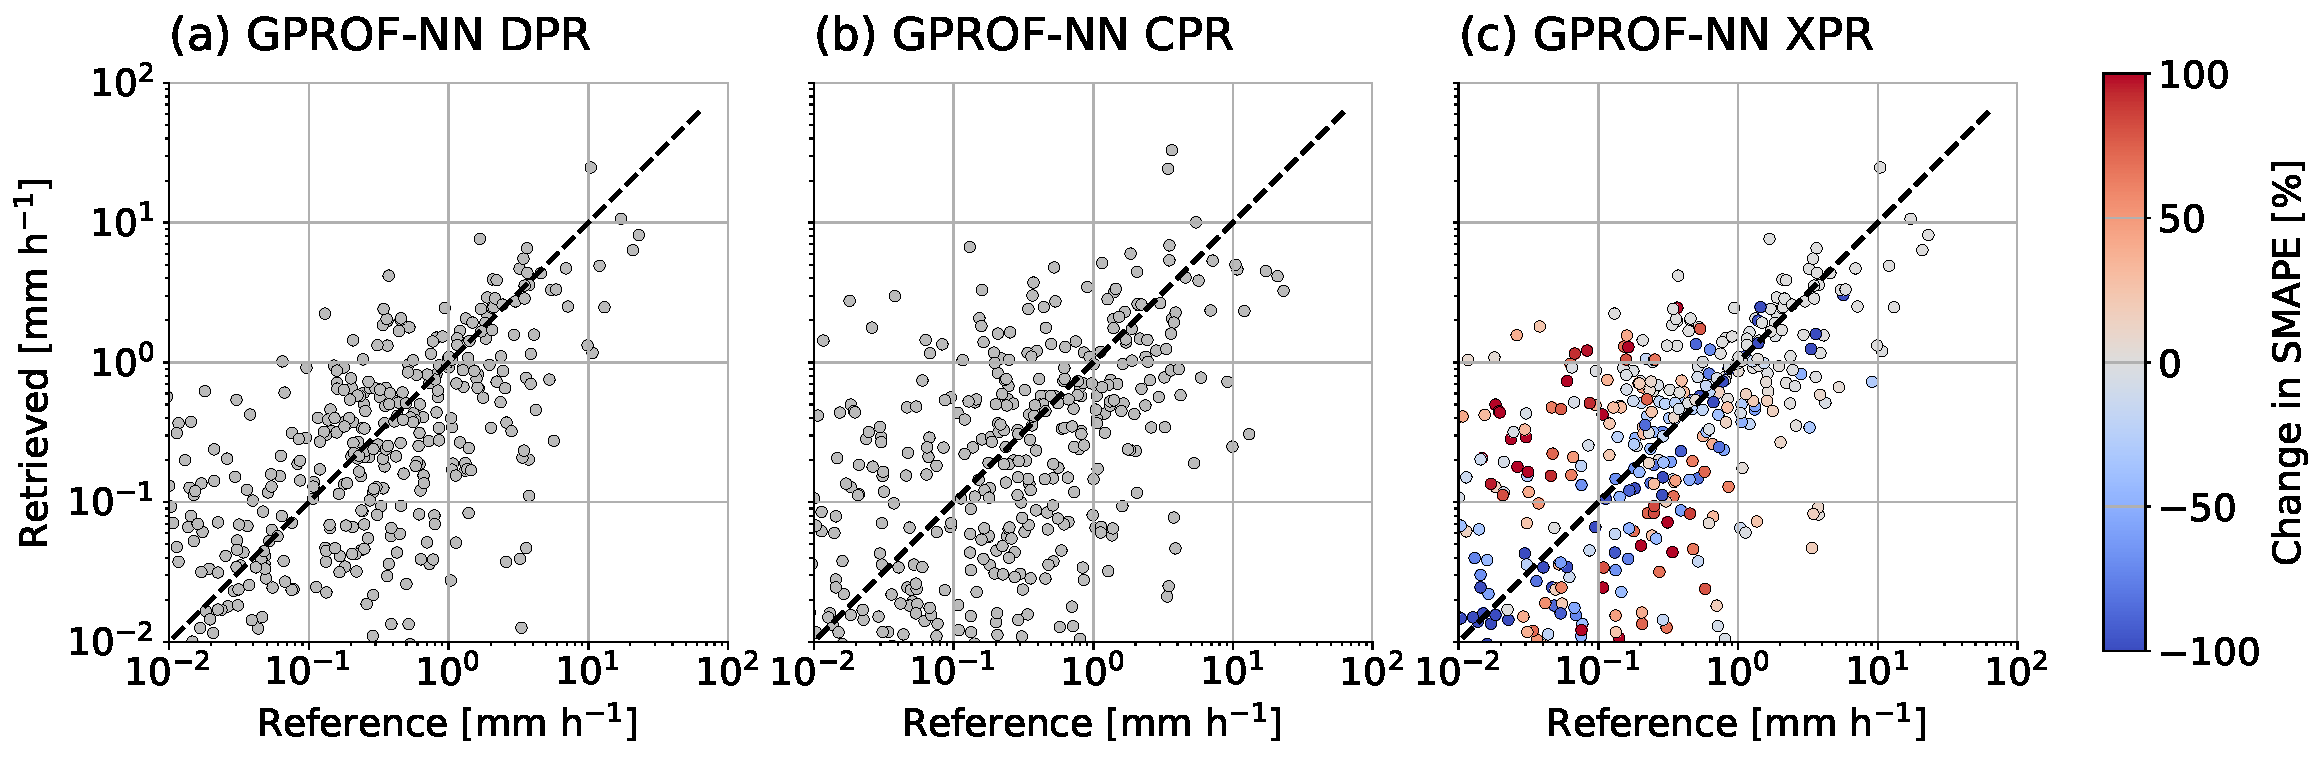
\includegraphics[width=37pc]{figures/figure09.pdf}}
 \caption{
 OceanRain measurements and matches GPROF-NN precipitation retrievals. Panels
 (a) – (c) display scatter plots of OceanRAIN reference precipitation and
 corresponding precipitation retrieved from the GPROF-NN DPR, GPROF-NN CPR, and
 GPROF-NN XPR retrievals. Shading in panel (c) indicates the change in the
 Symmetric Mean Percentage Error resulting from the merging of the DPR- and CPR-
 based estimates relative to the GPROF-NN DPR baseline.
 }\label{fig:ocean_rain_scatter}
\end{figure}

A statistical evaluation of the OceanRAIN overpasses is presented in Fig.~\ref{fig:ocean_rain_stats}.
Evaluated over all overpasses, both the DPR- and CPR-based estimates are biased
low. The bias of the DPR-based estimates is around 10 \%, while the DPR-based
estimates are biased low by 7 \%. Fusing the two estimates leads to a reduction
in bias to a positive bias of about 1 \%. At mid- and high latitudes, the low
bias of the DPR estimates is enhanced while the CPR estimates are biased high
with 16 \%. The fused precipitation estimates are biased low by about 7 \%. For
frozen precipitation, the bias in the DPR-based estimates increases to 51 \%
while the CPR-based estimates are low by 20 \%. The bias in the fused GPROF-NN
XPR precipitation estimates is -20 \%, similar to that of the CPR-based
estimates. The fusion of the DPR- and CPR- based estimates thus helps to reduce
systematic underestimation of the DPR-based retrieval. Furthermore, the biases
are smaller than for the GPROF V7 baseline as well as the ERA5 baseline except
for frozen precipitation.

In terms of instantaneous retrieval error, the CPR-based estimates have higher
errors than the DPR-based estimates, particularly at mid to high latitudes. The
fused estimates dampen these errors to some extent but remain higher or at the
level of the DPR-based estimates. The GPROF-NN XPR retrieval generally achieves
lower mean absolute and mean squared error than the ERA5 baseline as well as
higher correlation. The GPROF V7 baseline has smaller mean squared error and
higher correlation coefficient for all overpasses. However, comparing the GPROF
estimates to the actual DPR-based reference estimates using the 1028 OceanRAIN
overpasses with valid 2BCMB reference precipitation estimates, the GPROF-NN DPR
estimates achieve a MSE of 0.26 (mm h$^{-1}$)$^2$ and a linear correlation
coefficient of 0.84 compared to 0.32 (mm h$^{-1}$)$^2$ and a linear correlation
of 0.8 for the GPROF V7 baseline. This indicates that these small accuracy
differences are likely due to statistical noise in the validation data.


\begin{figure}[h]
 \centerline{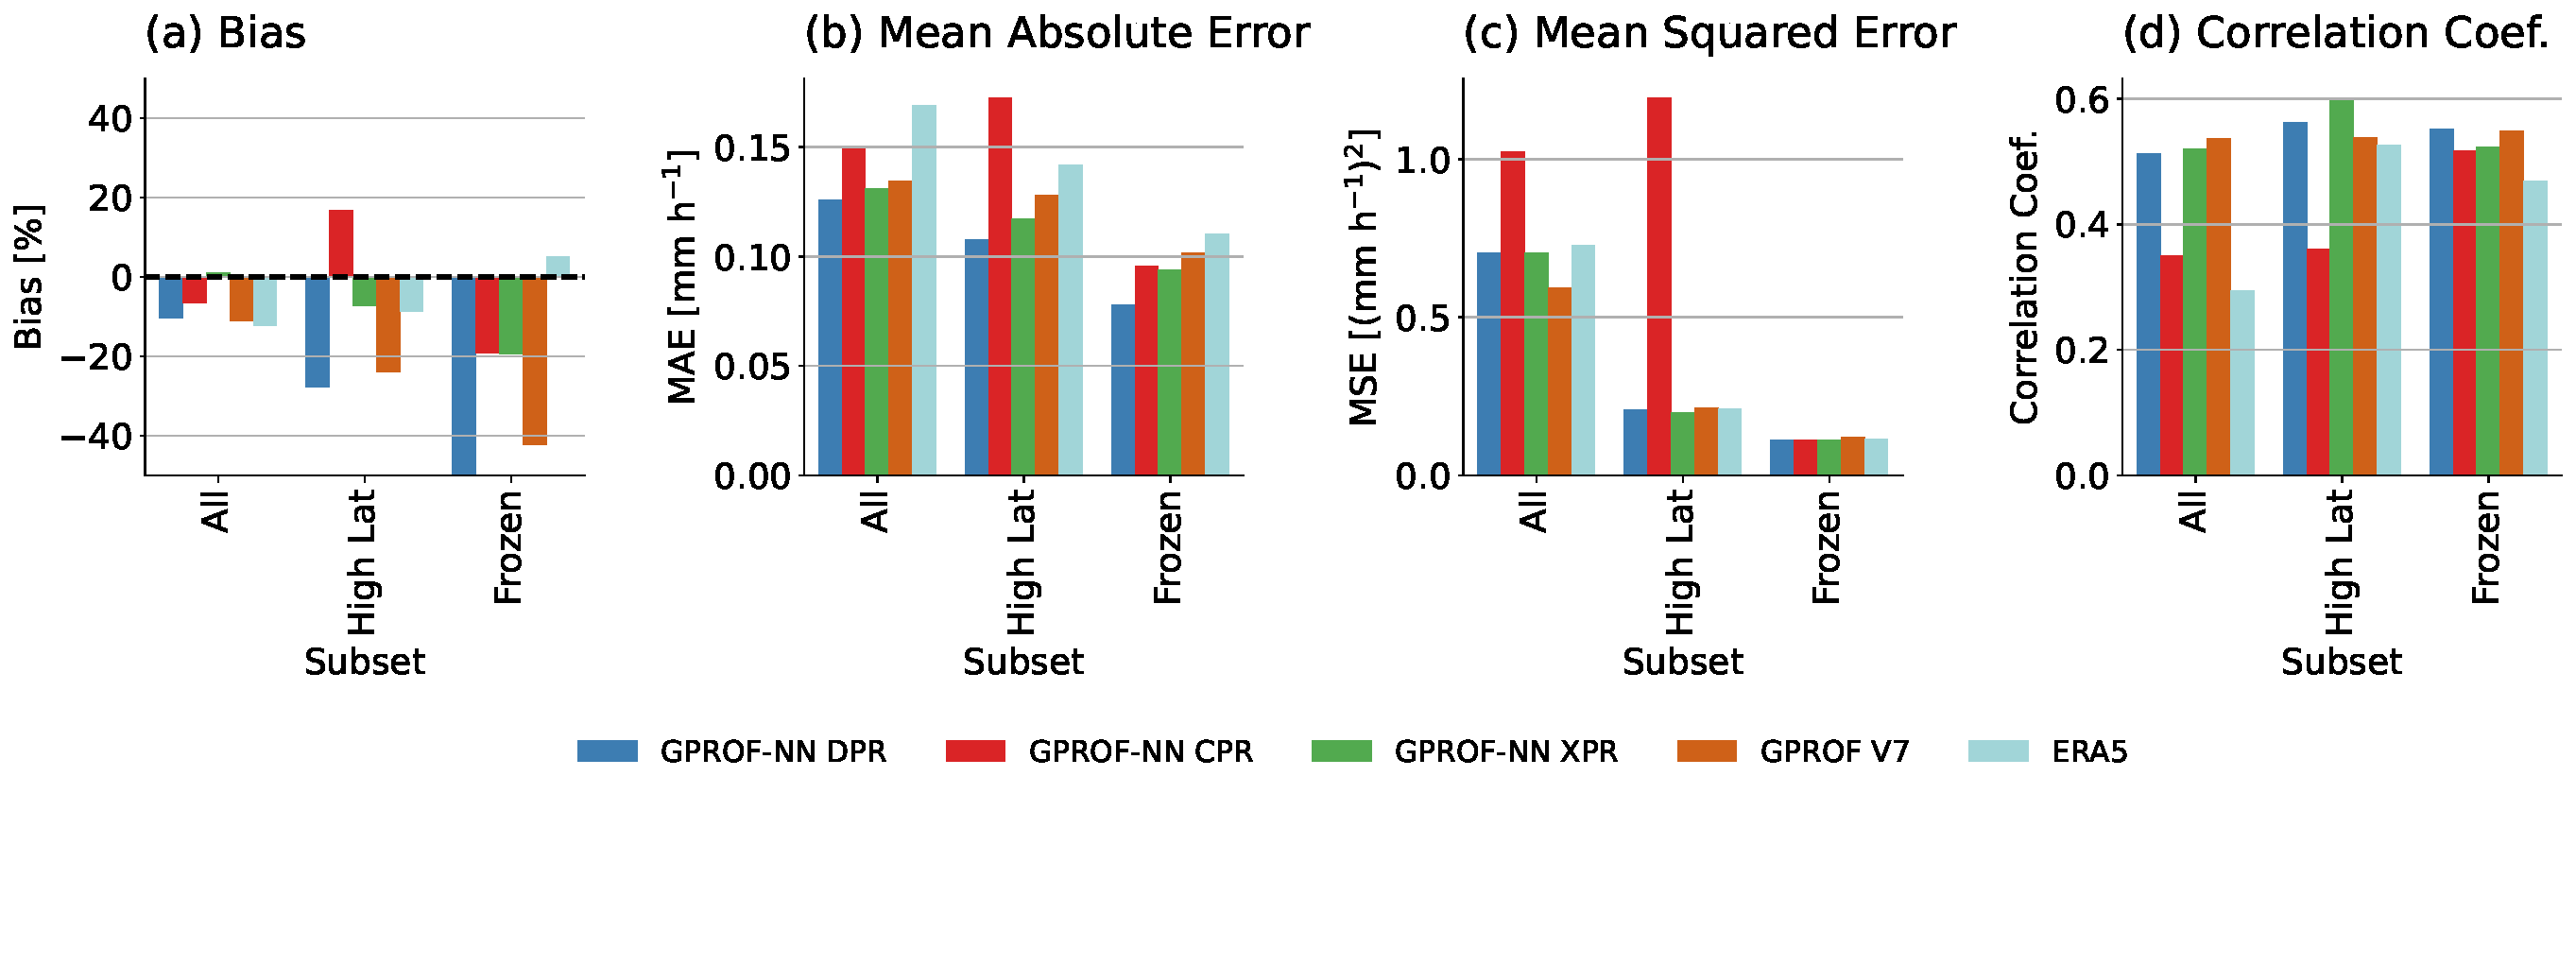
\includegraphics[width=37pc]{figures/figure10.pdf}}
 \caption{
Statistical evaluation of the GPROF-NN and baseline datasets against shipborne
in-situ measurements from the OceanRAIN dataset. Panels (a) – (d) display bias,
mean absolute error, mean squared error, and linear correlation coefficient for
GMI overpasses over the OceanRAIN vessels. Results are reported independently
for all overpasses (All), overpasses poleward of 45 deg (High Lat) and
overpasses with an estimated fraction of frozen precipitation exceeding 50
\% (Frozen).
 }\label{fig:ocean_rain_stats}
\end{figure}

\subsection*{Validation of CPR- and DPR-based Precipitation Estimates}

The validation against OceanRAIN shipborne distrometer measurements has shown
that the fusion of CPR- and DPR-based precipitation estimates improves the
precipitation detection skill and reduces systematic underestimation but
increases the random errors in the precipitation estimates. Assessment of the
CPR- and DPR-based estimates showed that these higher errors originate from the
CPR-based estimates, which exhibit significantly larger random errors than the
DPR-based estimates. Below we therefore examine CPR- and DPR-based precipitation
errors against independent estimates from ground-based radars.

Figure~\ref{fig:mrms_scatter} displays scatter plots of the CPR- and DPR-based
precipitation estimates compared to ground-based radar measurements. The
CPR-based precipitation estimates exhibit very high scatter compared to the
MRMS-based measurements particularly for MRMS precipitation rates up to 1 mm/h.
This is surprising given that the CloudSat estimates are expected to be more
reliable at low precipitation rates, where the radar observations are less
affected by attenuation. Nonetheless, the estimates achieve a correlation of 0.4
likely due to the better agreement for MRMS precipitation rates exceeding 1 mm
h$^{-1}$. The scatter plot indicates a distinct bi-modal behavior for MRMS
precipitation rates less than 1 mm h$^{-1}$, where the retrieval tends to either
heavly overestimate or underestimate the MRMS precipitation rates but almost
never matches them.

The DPR-based estimates show better agreement with the MRMS estimates.
Although the DPR based estimates strongly overestimate any MRMS estimates below
0.5 mm/h, which is a result of the limited sensitivity of the DPR, they
DPR-based estimates show very good agreement with the MRMS-based estimates for
precipitation rates from 5--10 mm/h, after which they start to exhibit a
tendency towards under-estimation.

\begin{figure}[h]
 \centerline{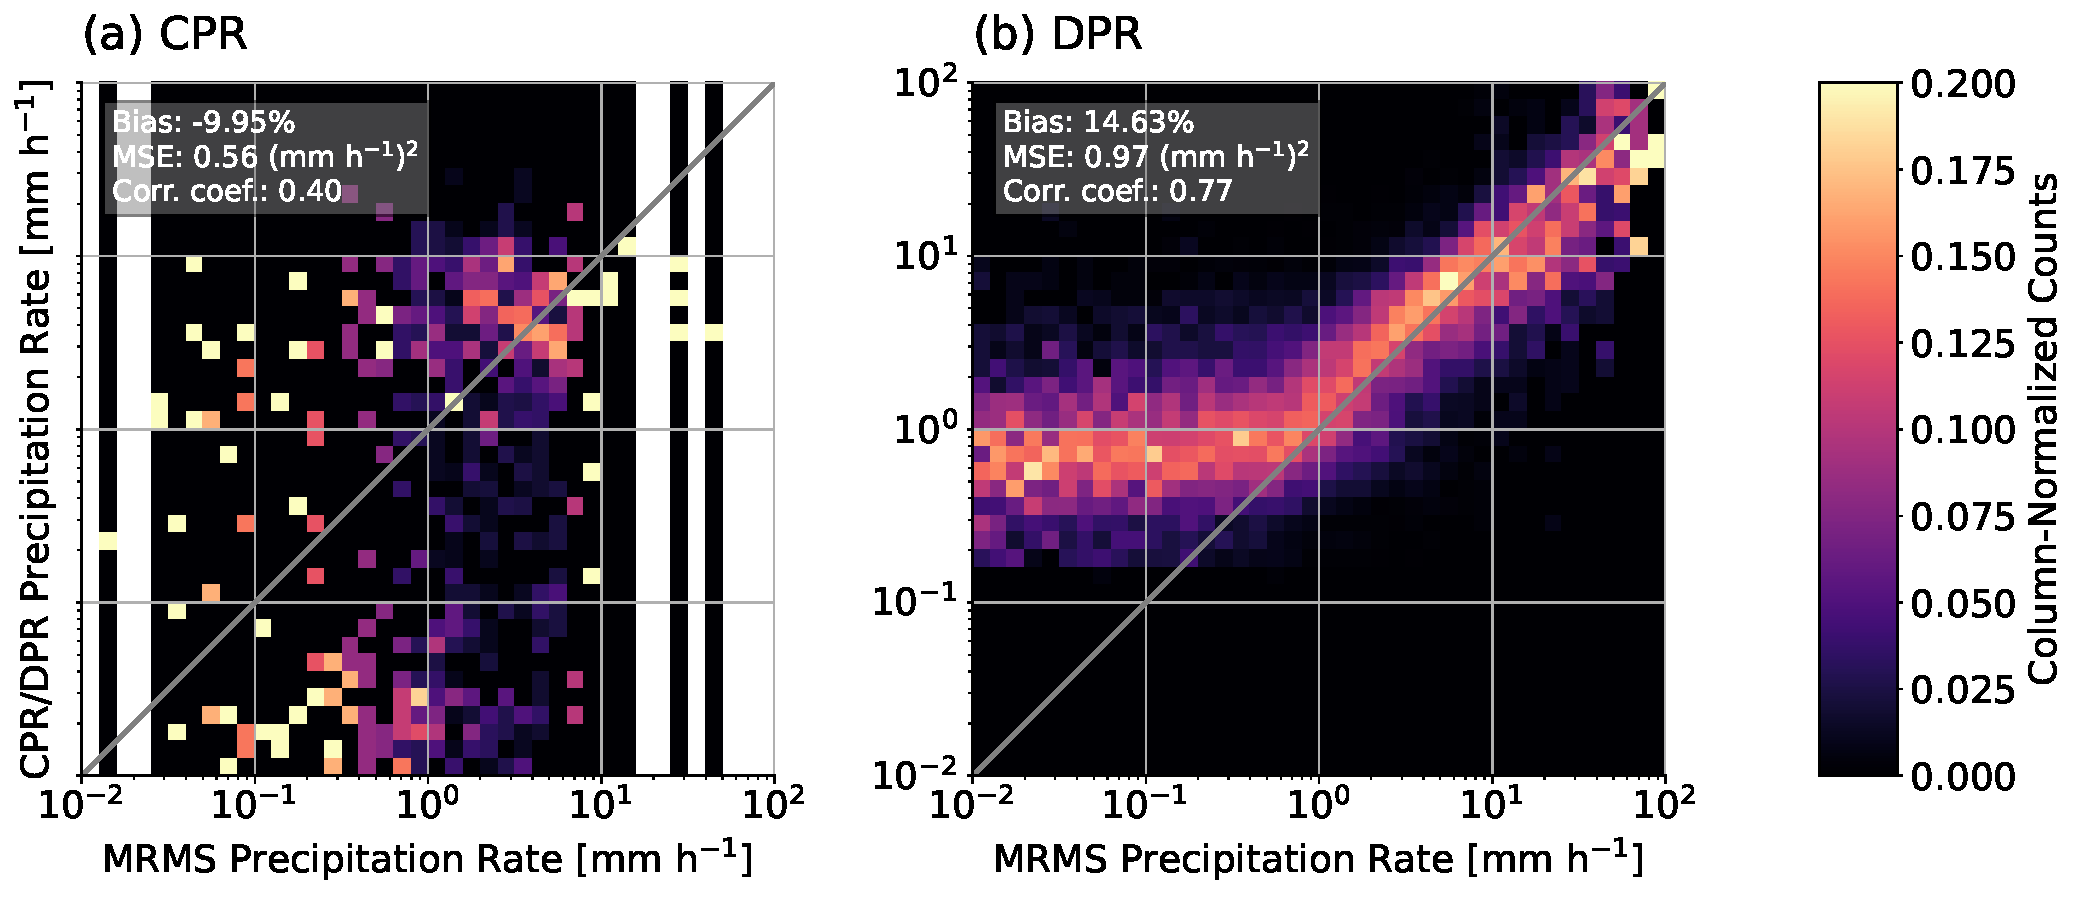
\includegraphics[width=37pc]{figures/figure11.pdf}}
 \caption{
Scatter plots of precipitation estimates from the (a) CPR- and (b) DPR-based
reference precipitation estimates compared to independent estimates from
ground-based radar.
 }\label{fig:mrms_scatter}
\end{figure}

To illustrate the likely failure mode of the CPR precipitation retrievals,
Figure~\ref{fig:mrms_case_study} shows one of the CPR overpasses from the
validation dataset. While the MRMS precipitation measurements indicate spatially
homogeneous with precipitation rates around 1 mm h$^{-1}$ throughout most of the
scene, the CPR-based precipitation oscillate between 0.01 and 10 mm h$^{-1}$.
The principal change in CPR radar reflectivities during the transition from 10
mm h$^{-1}$ to 0.01 mm h$^{-1}$ is a strong increase in the surface backscatter
while the above-surface reflectivities remain relatively similar. While limited,
this evidence suggest that the errors in the CPR-based precipitation estimates
may be related to the handling of the surface backscatter rather than inherent
limitations of the radar observations.


\begin{figure}[h]
 \centerline{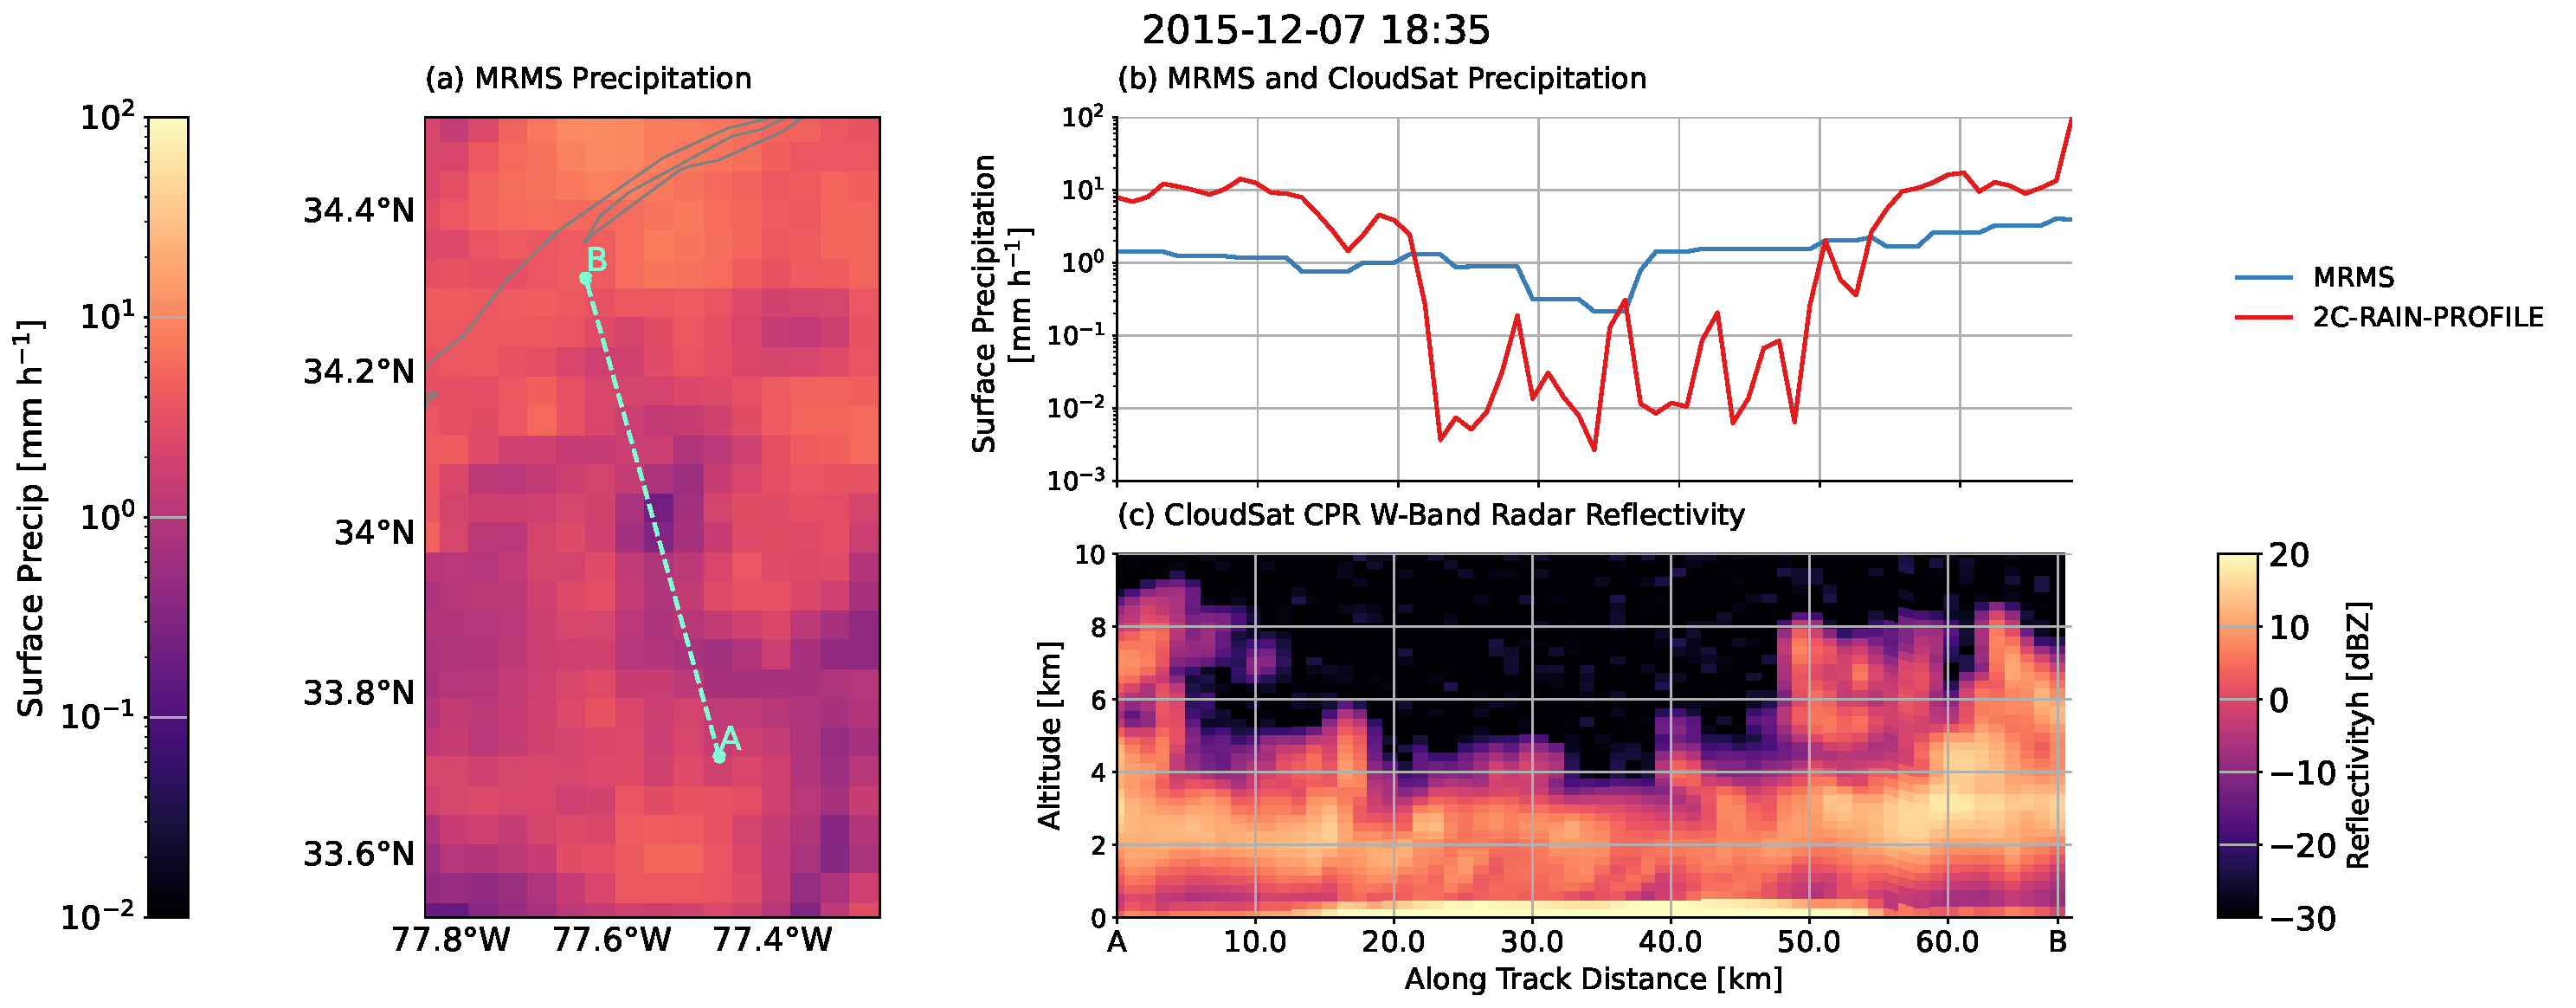
\includegraphics[width=37pc]{figures/figure12.pdf}}
 \caption{
   Comparison of collocated CPR and MRMS precipitation estimates. Panel (a)
   displays the MRMS precipitation field and the ground track of the CPR
   observations. Panels (b) and (c) display the MRMS and CPR precipiation rates
   and the CPR radar reflectivity along the track, respectively.
 }\label{fig:mrms_case_study}
\end{figure}

The comparison against the independent precipitation estimates from MRMS
indicates that the CPR-based precipitation estimates do not yield an accurate
quantitative estimate of light precipitation. In particular, the retrieval seems
to exhibit a tendency to either strongly underestimate or strongly overestimate
the MRMS precipitation within the range of 0.1 to 1 mm/h. As shown in
Fig.~\ref{fig:cpr_cmb_scatter}, this behavior is also observed when the CPR
estimates are directly compared to the DPR-based estimates. Although one would
expect the CPR and DPR estimates to agree across precipitation estimates from
0.5 to 1 mm/h, these results confirm that there is no consistency between the
precipitation estimates within this range. The results in Fig. 11 further show
that the inconsistency between the estimates is largely caused by the
precipitation estimates from the 2C-Rain-Profile product. The snowfall estimates
from the 2C-Snow-Profile product show some consistency for estimates around 1
mm/h.

\begin{figure}[h]
 \centerline{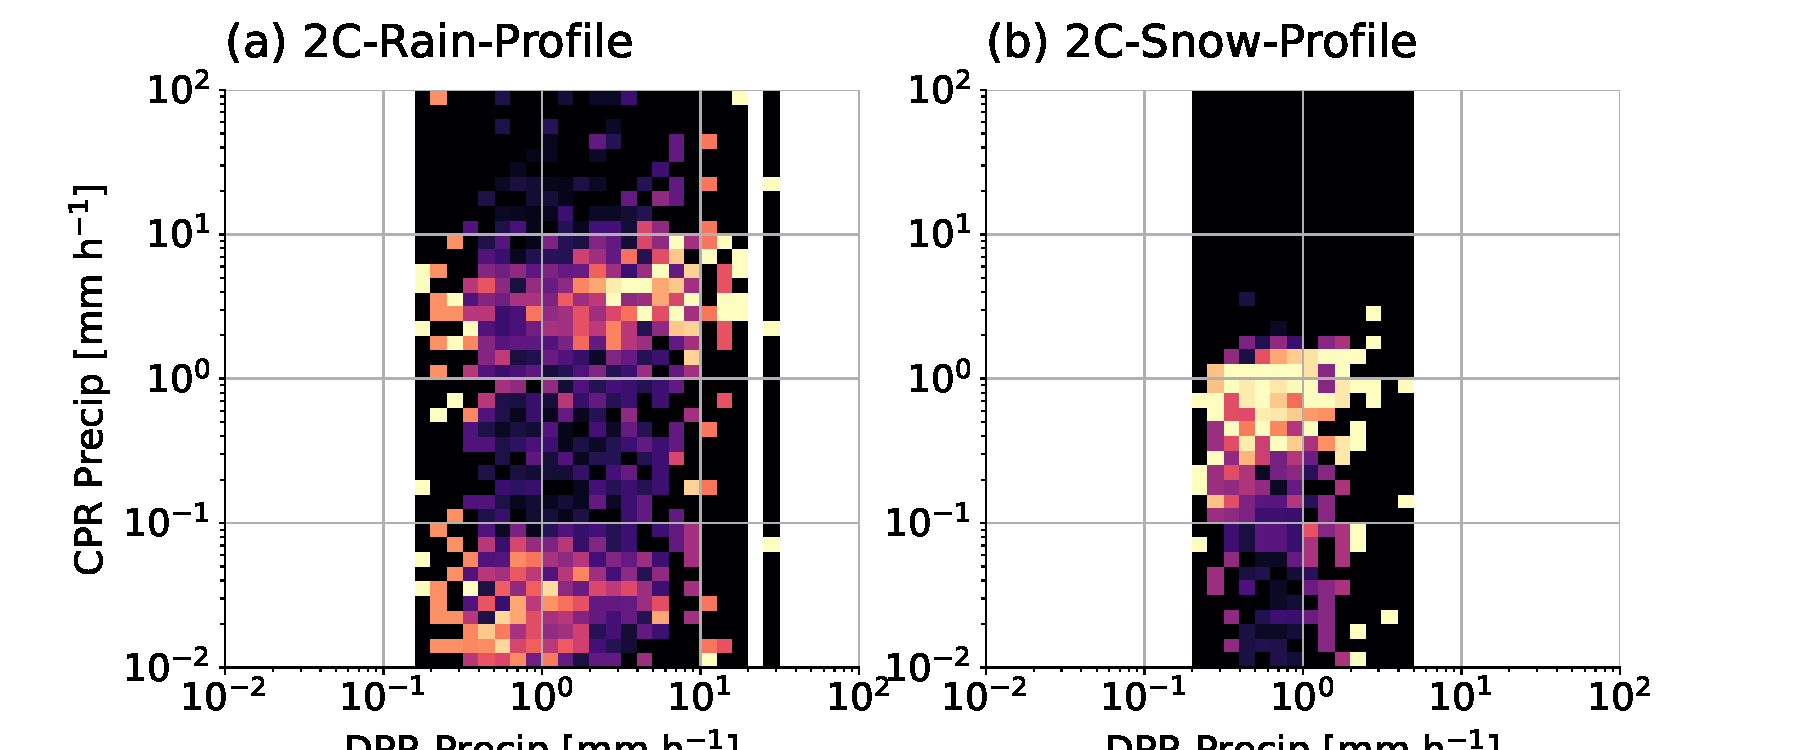
\includegraphics[width=37pc]{figures/figure13.pdf}}
 \caption{
Scatter plot comparing CPR- and DPR- based precipitation estimates. Panel (a)
compares the DPR-based precipitation estimates from the GPM 2BCMB product with
estimates of the CloudSat 2C-Rain-Profile product. Panel (b) compares the GPM
estimates with snowfall estimates from the 2C-Snow-Profile product.
 }\label{fig:cpr_cmb_scatter}
\end{figure}

\subsection{Global Precipitation Distributions}

Although the fusing of CPR- and DPR- based precipitation estimates does not
increase the accuracy of individual precipitation estimates, it has shown clear
improvements in precipitation detection and reductions of climatological biases
compared to shipborne distrometer measurements indicating that the fused CPR–DPR
estimates better represent light and frozen precipitation. Below we characterize
the impact of fusing CPR and DPR-based precipitation estimates on global
precipitation distributions.

Figure~\ref{fig:zonal_means_all} displays the zonal distribution of ocean precipitation as retrieved by
the GPROF-NN CPR, DPR, and XPR retrievals. The CPR-based retrieval yields higher
precipitation rates poleward of the mid-latitude storm tracks but severely
underestimate precipitation in the tropics and extratropics compared to the
estimates derived from DPR-based retrieval. The fused estimates track the GPM
DPR-based estimates within -30 and 30 degree N. Starting at 40 N and -30 degree
North, the fused estimates follow closer to the CPR-based precipitation
estimates.

\begin{figure}[h]
 \centerline{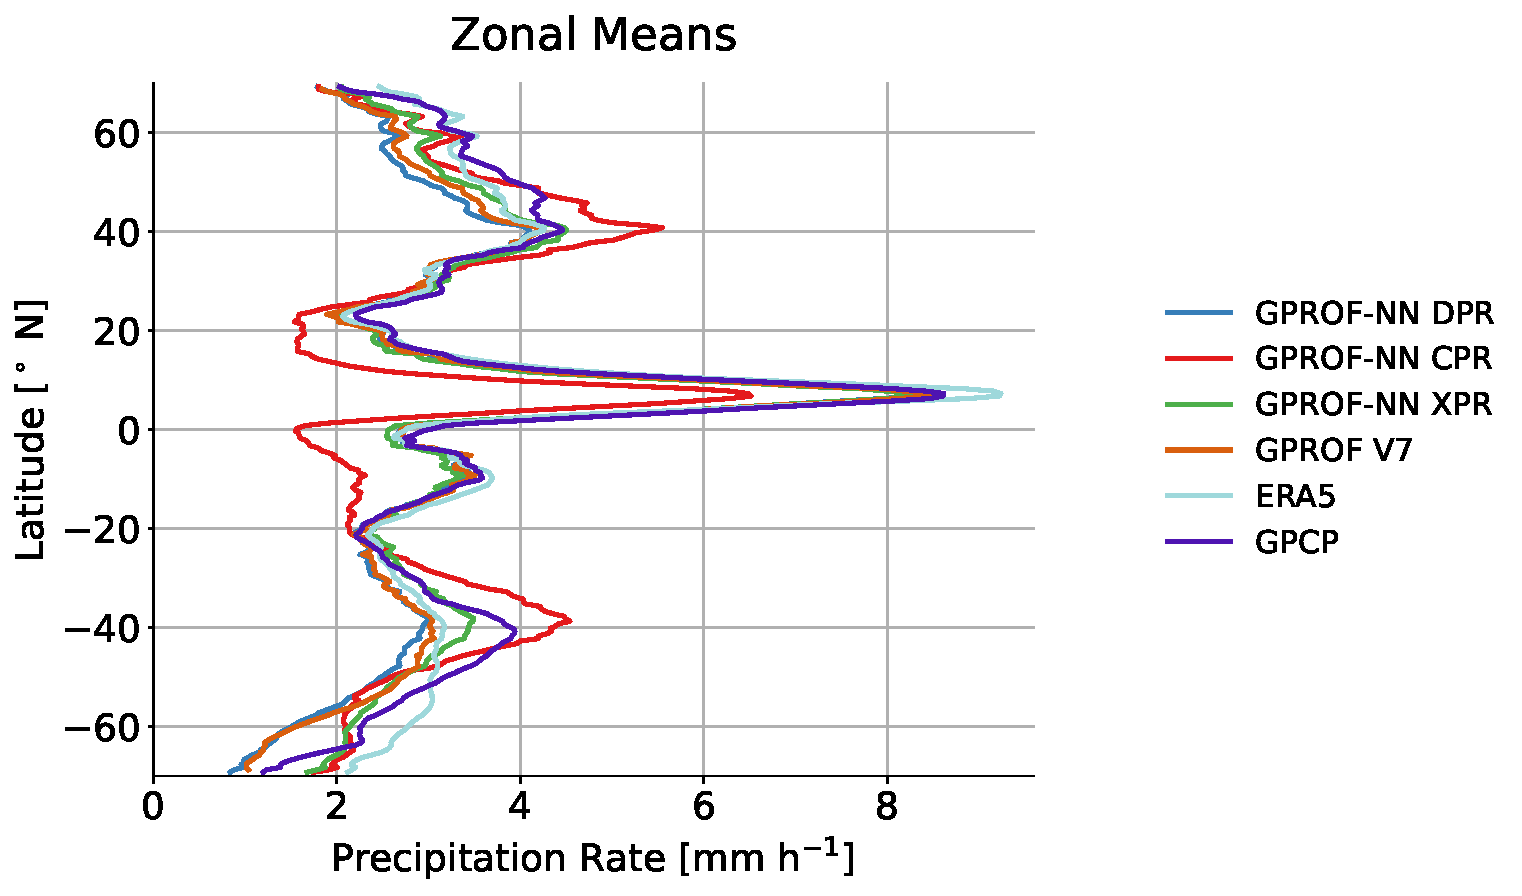
\includegraphics[width=37pc]{figures/figure14.pdf}}
 \caption{
Zonal means of oceanic precipitation estimates. The figure compares estimates
from the CPR-based (GPROF-NN CPR), the DPR-based (GPROF-NN DPR), and from the
fused precipitation estimates (GPROF-NN XPR) to reference estimates from GPROF V07, ERA5,
and GPCP.
 }\label{fig:zonal_means_all}
\end{figure}

The global retrieved distributions are displayed in
Fig.~\ref{fig:global_means_all}. Compared to the DPR-based retrievals, the
CPR-based estimates add more than 2 mm per day over the storm tracks and
high-latitude oceans. The fused XPR estimates add precipitation over the storm
tracks and high latitudes albeit less than the CloudSat-based retrieval alone.
The fused precipitation estimates slightly decrease precipitation over the
Indian ocean and West Pacific but increase it over the eastern Pacific.

ERA5 exhibits higher precipitation rates than the DPR-based reference retrievals
almost everywhere. However, pockets of decreasing precipitation are visible in
the Indian Ocean and the West Pacific roughly matching areas of decreasing
precipitation in the GPROF-NN XPR results. GPCP precipitation rates are also
globally higher with scattered regions of decreasing precipitation.


\begin{figure}[hp]
 \centerline{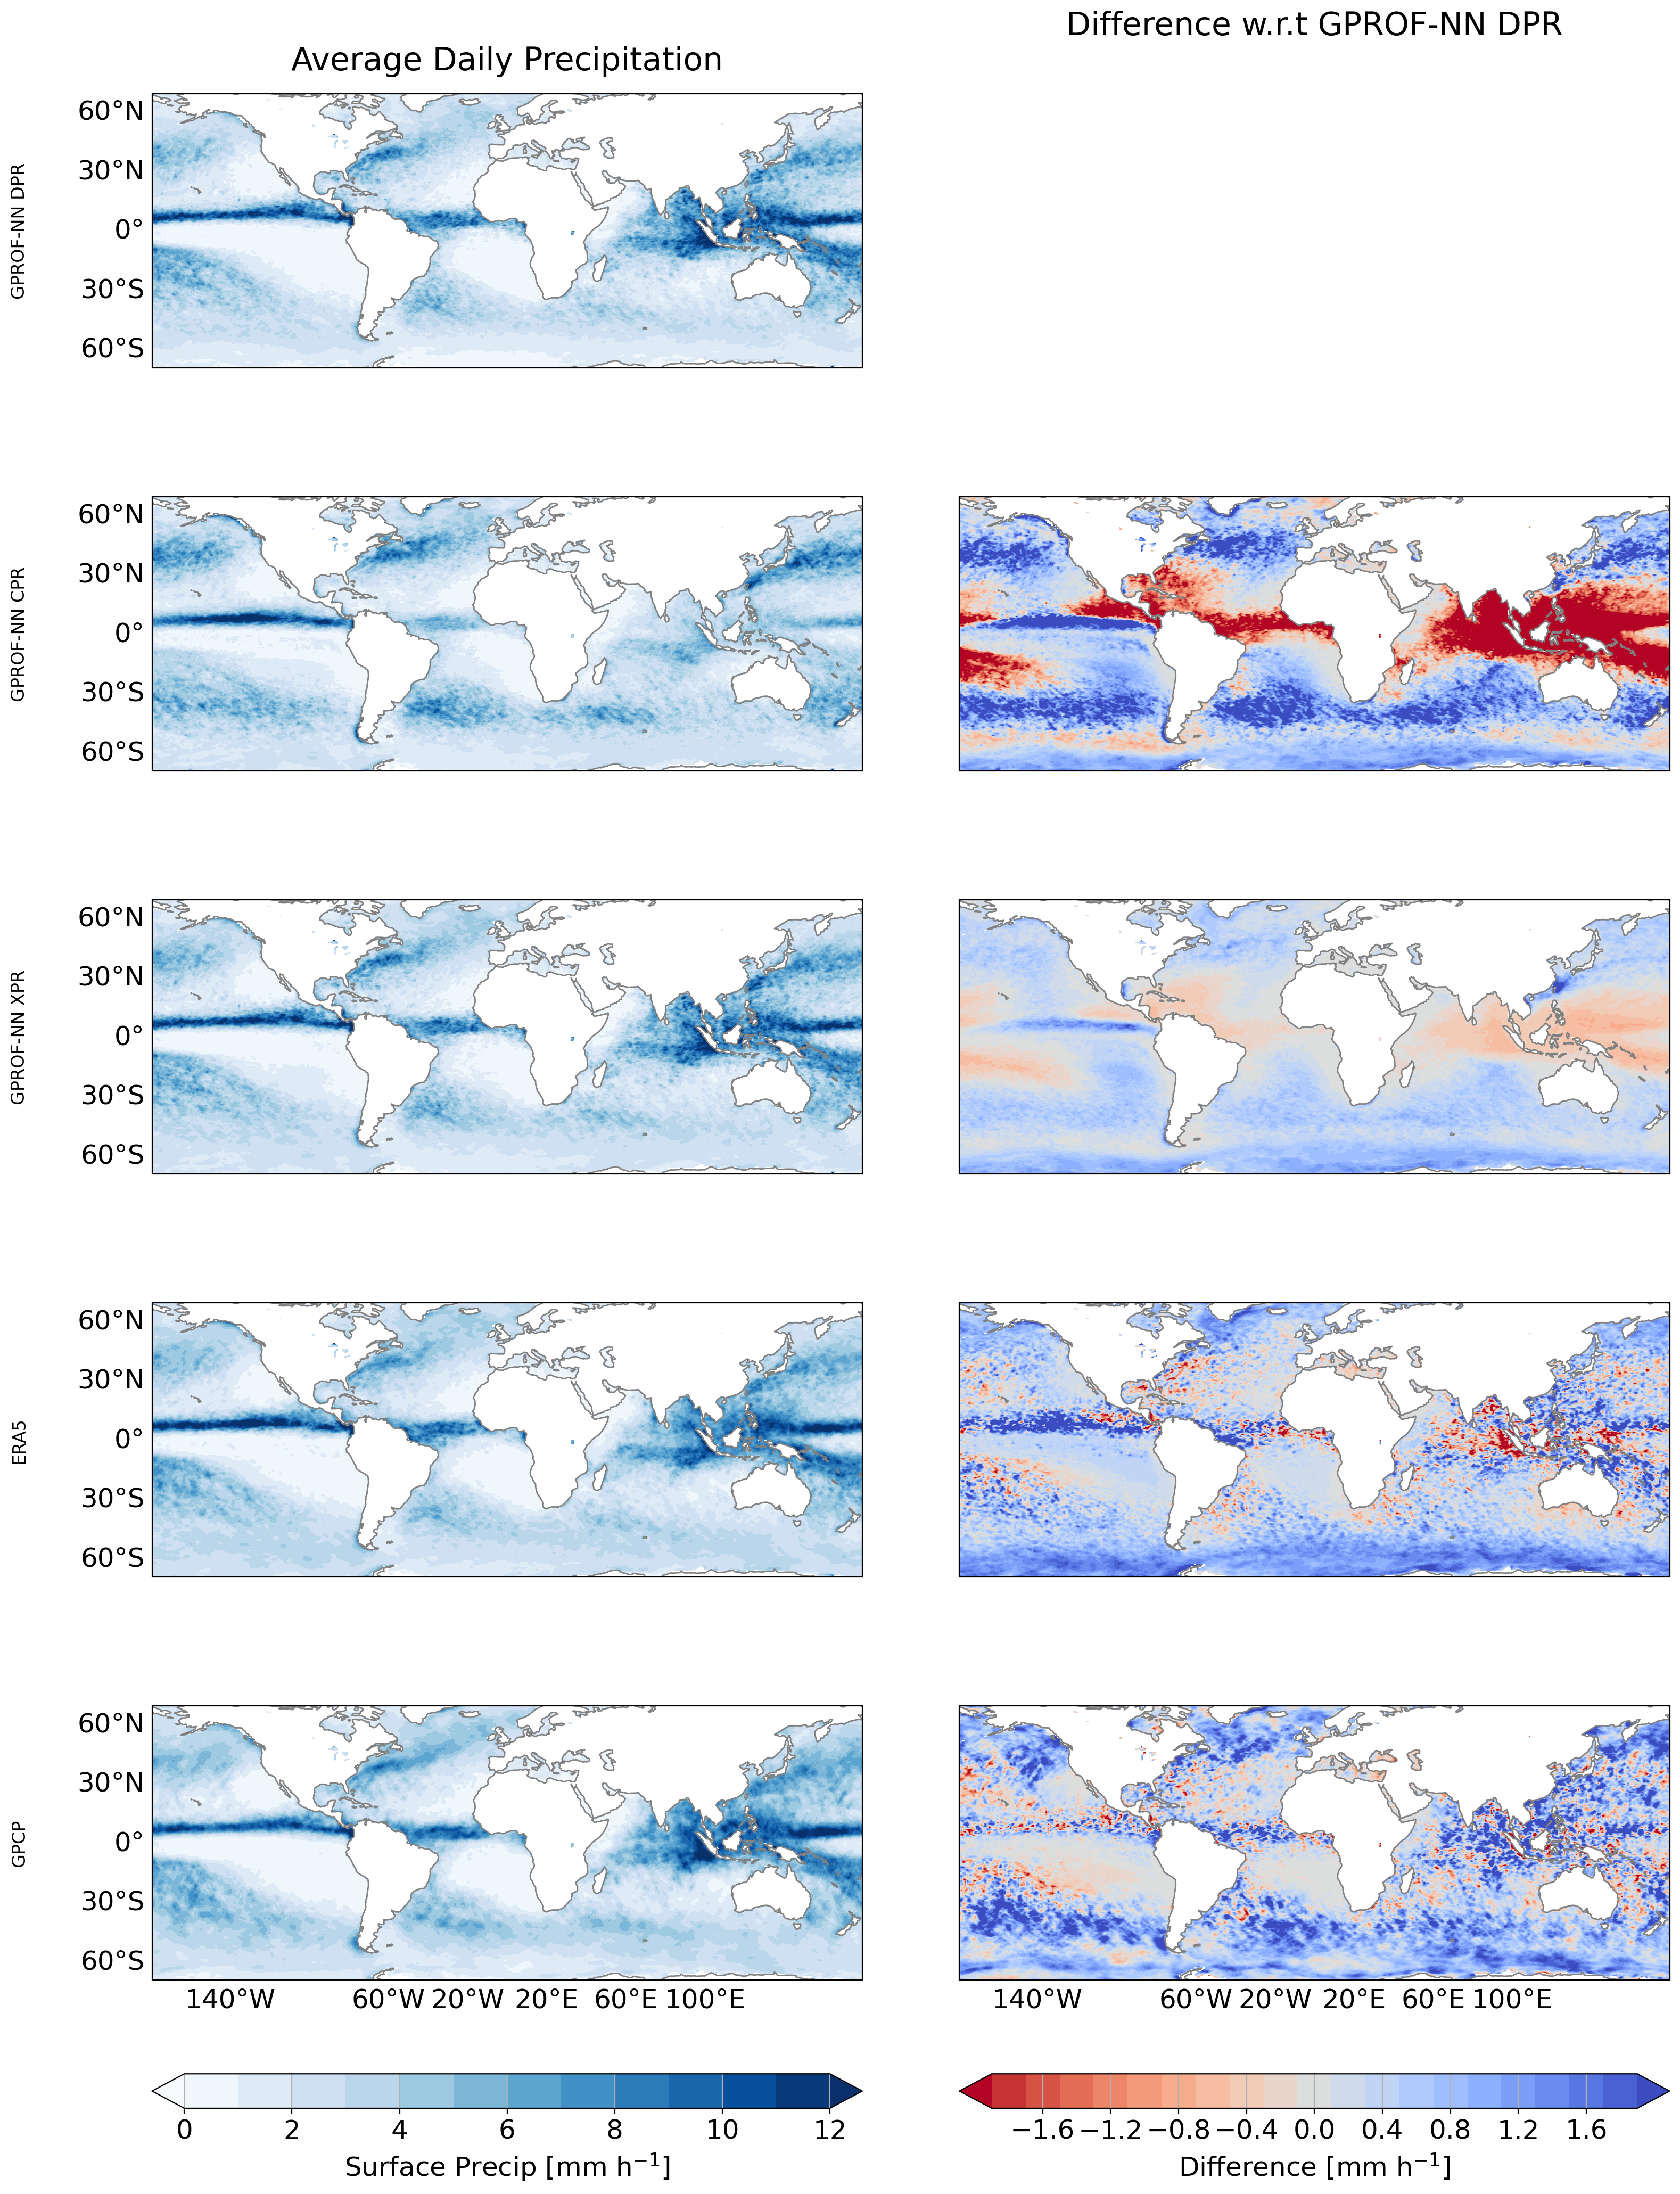
\includegraphics[width=37pc]{figures/figure15.png}}
 \caption{
Global distributions of mean daily precipitation accumulations from the DPR-based estimates (GPROF-NN DPR), the CPR-based estimates (GPROF-NN CS), and the merged estimates (GPROF-NN XPR) and the ERA5 and GPCP datasets.
 }\label{fig:global_means_all}
\end{figure}

\section{Summary and Conclusions}
\label{sec:summary}

This work presents GPROF-NN XPR, a novel precipitation retrieval aimed to
overcome limitations of current global PMW precipitation retrievals imposed by
shortcomings of the reference data used to train machine-learning-based
algorithms. The retrieval combines dedicated estimates of light precipitation
based on reference data from the CloudSat CPR with general precipitation
estimates based on reference data from the GPM DPR. A simple fusion scheme is
proposed to combine the light and regular precipitation estimates into a single
fused precipitation estimate.

Validation of the fused GPROF-NN XPR precipitation estimates shows improved
precipitation detection and a reduction of the systematic underestimation that
commonly affects retrievals, particularly at high latitudes and for frozen
precipitation. These results indicate that GMI PMW observations can help bridge
the current sensitivity gap between precipitation measurements from the CloudSat
and DPR missions. By providing more direct estimates of precipitation across a
wide range of precipitation and climate regimes, the GPROF-NN XPR retrieval
therefore has the potential to improve the representation of precipitation in
global precipitation datasets. In particular, it may reduce the need for
climatological corrections that suppress monthly and interannual variability in
such datasets.

These findings also highlight the potential for more effective synergistic
active–passive precipitation retrievals using GMI observations. The DPR-based
estimates used here are derived from the GPM 2BCMB product, which already
combines radar and radiometer information. However, the current algorithm only
retrieves precipitation where the radar observations indicate hydrometeor
backscatter. The results presented here demonstrate that GMI observations alone
can identify precipitation that is not detected by the DPR, suggesting that
current combined radar–radiometer retrievals do not yet fully exploit the
synergistic potential of the active and passive microwave observations provided
by the GPM satellite. Although the fused precipitation estimates improve
detection and reduce climatological biases, the fusion increases random
retrieval errors compared to the DPR-based estimates. Validation of the
CPR-based precipitation estimates from the 2C-Rain-Profile product provide more
sensitive but generally less accurate quantitative precipitation estimates than
the DPR-based reference. The comparison against both ground-based radar and
against DPR show large spread at light precipitation rates with a bi-modal
tendency to either strongly underestimate or overestimate precipitation by an
order of magnitude. The bi-modal behavior of the 2C-Rain-Profile was already
noted in the first publication describing the retrieval but apparently has not
been further investigated since. This is concerning considering the
2C-Rain-Profile estimates are used to calibrate principal global precipitation
products including IMERG and GPCP.

The extensive validation of the GPROF-NN XPR estimates provided here confirms
that the fused precipitation estimates improve the representation of light and
frozen precipitation despite the discovered inconsistencies in the CPR-based
precipitation estimates. The GPROF-NN XPR retrieval will therefore be used as an
auxiliary retrieval to add light precipitation to the DPR-based reference data
that will be used to train the retrieval algorithms for the next operational
version of the GPM PMW retrieval algorithms.

While the GPROF-NN XPR estimates constitute an additional step towards improved
global estimates of oceanic precipitation from the GPM missions, this work
highlights remaining challenges of current global precipitation products. Since
CPR- and DPR-based are currently used in combination to calibrate global
precipitation products, it should be ensured that these products are consistent
across the shared sensitivity range of CPR and DPR. Moreover, our results
indicate that current synergistic active–passive precipitation retrievals
underutilize passive observations and could likely be improved to overcome
limitations of current active sensors.



Citations to standard references in text should consist of the name of the
author and the year of publication, for example, \citet{Becker+Schmitz2003} or
\citep{Becker+Schmitz2003} using the appropriate $\backslash$citet\ or
$\backslash$citep commands, respectively. A variety of citation formats can
be used with the natbib package; however, the AMS prefers that authors use only the $\backslash$citet\ and
$\backslash$citep commands. References should be entered in the references.bib file. For a thorough
discussion of how to enter references into the references.bib database file
following AMS style, please refer to the \textbf{AMS\_RefsV6.pdf} document
included in this package.

\section{Formatting math}
The following sections will outline the basic formatting rules for
mathematical symbols and units.  In addition, a review of the amspaper.tex
file will show how this is done with the use of \LaTeX\ commands.  The AMS
template provides the American Mathematical Society math, font, symbol, and
boldface packages for use in math mode.

\subsection{Mathematical symbols}
Symbols must be of the same font style both in text discussion and in
displayed equations or terms (and figures should be prepared to match).
Scalar single-character symbols are set italic, Greek, or script. Examples
are $u$, $L$ [note that $\upsilon$ (Greek upsilon) is used instead of
\textit{v} (italic ``vee'') to avoid confusion with $\nu$ (Greek nu) often
used for viscosity; this is handled automatically when in \LaTeX\ math mode],
$w$, $x$, $y$, $z$, $f$, $g$, $r$, indices such as $i$ or $j$, and constants
such as $C_D$, $k$, or $K$. Multiple-character scalar variables,
abbreviations, nondimensional numbers, and acronyms for variables are set
regular nonitalic: $\mathrm{LWC}$, $\mathrm{Re}$, $\mathrm{Ro}$,
$\mathrm{BT}$, $\mathrm{abs}$, $\mathrm{obs}$, $\mathrm{max}$,
$\mathrm{min}$, $\mathrm{Re}$/$\mathrm{Im}$ (real/imaginary), etc. For
vectors, use boldface nonitalic Times Roman as in $\mathbf{V}$, $\mathbf{v}$,
or $\mathbf{x}$, and $\mathbf{i}$, $\mathbf{j}$, and $\mathbf{k}$ unit
vectors. Do not use the \LaTeX\ $\backslash$vec command to denote vectors.
For matrix notation, use nonitalic boldface Arial (or sans serif) font as in
$\bm{\mathsf{A}}$, $\bm{\mathsf{B}}$, or $\bm{\mathsf{M}}$.  All mathematical
operator abbreviations/acronyms are set lowercase regular Roman font, except
$O$ (on the order of): $\sin$, $\cos$, $\tan$, $\tanh$, $\mathrm{cov}$, $\Pr$
(for probability; note same as Prandtl number), $\mathrm{const}$ (for
constant), $\mathrm{c.c.}$ (complex conjugate).

\subsection{Units}
Units are always set on a single line with a space separating the
denominator, which is set with a superscript $-1$, $-2$, and so on, rather
than using a slash for ``per.'' Examples are g kg$^{-1}$, m$^2$ s$^{-1}$, W
m$^{-2}$, g m$^{-3}$, and m s$^{-1}$ (note that ms$^{-1}$ is the unit for
``per millisecond'').

\subsection{Equations}
Brief equations or terms set inline in text must be set as a single-line
expression because page proofs are not double spaced, for example,
$\rho^{-1}p/x$ or $(1/{\rho})p/x$ or $(a-b)/(c+d)$; that is, use a
superscript $-1$ for the denominator. In case of a more complicated term or
equation, it should be set as an unnumbered display equation, such as
\begin{displaymath} x=\frac{2b\pm\sqrt{b^{2}-4ac}}{2c}.  \end{displaymath}

Otherwise, numbered display equations can be entered using the appropriate
equation command, such as \begin{equation}
x=\frac{2b\pm\sqrt{b^{2}-4ac}}{2c}.  \end{equation}

Lists of equations are punctuated as written English, and commas, semicolons,
and periods are placed where appropriate. Conjunctions such as ``and,''
``while,'' ``when,'' or ``for'' are also typically placed before the final
element in a mathematical phrase, as befits the intended mathematical
meaning.  

\section{Figures and tables}

\subsection{Figures}
The insertion of a sample figure (Fig. \ref{f1})  
and caption is given below (in the .tex document). Standard figure sizes are 19 (one column), 
27, 33, and 39 (two columns) picas.

\begin{figure}[h]
 \centerline{
\includegraphics[width=19pc]{figure01.pdf}}
  \caption{Enter the caption for your figure here.  Repeat as
  necessary for each of your figures. Figure from \protect\cite{Knutti2008}.}\label{f1}
\end{figure}


\subsection{Tables}
Each table must be numbered, provided with a caption, and mentioned
specifically in the text. See below for sample table formatting (Tables \ref{t1} and \ref{AT1}).

\begin{table}[h]
\caption{This is a sample table caption and table layout.}\label{t1}
\begin{center}
\begin{tabular}{ccccrrcrc}
\topline
$N$ & $X$ & $Y$ & $Z$\\
\midline
 0000 & 0000 & 0010 & 0000 \\
 0005 & 0004 & 0012 & 0000 \\
 0010 & 0009 & 0020 & 0000 \\
 0014 & 0010 & 0029 & 0005 \\
\botline
\end{tabular}
\end{center}
\end{table}

%%%%%%%%%%%%%%%%%%%%%%%%%%%%%%%%%%%%%%%%%%%%%%%%%%%%%%%%%%%%%%%%%%%%%
% TABLES---INSERT NEAR IN-TEXT DISCUSSION
%%%%%%%%%%%%%%%%%%%%%%%%%%%%%%%%%%%%%%%%%%%%%%%%%%%%%%%%%%%%%%%%%%%%%
%% Enter tables near where they are discussed within the document.
%%
%
%\begin{table}[h]
%\caption{This is a sample table caption and table layout.  
%Table from Lorenz (1963).}\label{t1}
%\begin{center}
%\begin{tabular}{ccccrrcrc}
%\topline
%$N$ & $X$ & $Y$ & $Z$\\
%\midline
% 0000 & 0000 & 0010 & 0000 \\
% 0005 & 0004 & 0012 & 0000 \\
% 0010 & 0009 & 0020 & 0000 \\
% 0015 & 0016 & 0036 & 0002 \\
% 0020 & 0030 & 0066 & 0007 \\
% 0025 & 0054 & 0115 & 0024 \\
%\botline
%\end{tabular}
%\end{center}
%\end{table}


%%%%%%%%%%%%%%%%%%%%%%%%%%%%%%%%%%%%%%%%%%%%%%%%%%%%%%%%%%%%%%%%%%%%%
% FIGURES---INSERT NEAR IN-TEXT DISCUSSION
%%%%%%%%%%%%%%%%%%%%%%%%%%%%%%%%%%%%%%%%%%%%%%%%%%%%%%%%%%%%%%%%%%%%%
%%  Enter figures near where they are discussed within the document.
%%
%
%\begin{figure}[t]
%  \noindent
\includegraphics[width=19pc,angle=0]{figure01.pdf}\\
%  \caption{Enter the caption for your figure here.  Repeat as
%  necessary for each of your figures. Figure from \protect\cite{Knutti2008}.}\label{f1}
%\end{figure}

\clearpage
%%%%%%%%%%%%%%%%%%%%%%%%%%%%%%%%%%%%%%%%%%%%%%%%%%%%%%%%%%%%%%%%%%%%%
% ACKNOWLEDGMENTS
%%%%%%%%%%%%%%%%%%%%%%%%%%%%%%%%%%%%%%%%%%%%%%%%%%%%%%%%%%%%%%%%%%%%%
\acknowledgments
Keep acknowledgments (note correct spelling: no ``e'' between the ``g'' and
``m'') as brief as possible. In general, acknowledge only direct help in
writing or research. Financial support (e.g., grant numbers) for the work done, 
for an author, or for the laboratory where the work was performed must be 
acknowledged here rather than as footnotes to the title or to an author's name.
Contribution numbers (if the work has been published by the author's institution 
or organization) should be placed in the acknowledgments rather than as 
footnotes to the title or to an author's name.

%%%%%%%%%%%%%%%%%%%%%%%%%%%%%%%%%%%%%%%%%%%%%%%%%%%%%%%%%%%%%%%%%%%%%
% DATA AVAILABILITY STATEMENT
%%%%%%%%%%%%%%%%%%%%%%%%%%%%%%%%%%%%%%%%%%%%%%%%%%%%%%%%%%%%%%%%%%%%%
% 
%
\datastatement
The data availability statement is where authors should describe how the data underlying 
the findings within the article can be accessed and reused. Authors should attempt to 
provide unrestricted access to all data and materials underlying reported findings. 
If data access is restricted, authors must mention this in the statement.
See http://www.ametsoc.org/PubsDataPolicy for more details.


%%%%%%%%%%%%%%%%%%%%%%%%%%%%%%%%%%%%%%%%%%%%%%%%%%%%%%%%%%%%%%%%%%%%%
% APPENDIXES
%%%%%%%%%%%%%%%%%%%%%%%%%%%%%%%%%%%%%%%%%%%%%%%%%%%%%%%%%%%%%%%%%%%%%

%% If only one appendix, use

%\appendix

%% If more than one appendix, use \appendix[<letter>], e.g.,

%\appendix[A] 

%% Appendix title is necessary! For appendix title:

%\appendixtitle{Title of Appendix}

%%% Appendix section numbering (note, skip \section and begin with \subsection)
%
% \subsection{First primary heading}

% \subsubsection{First secondary heading}

% \paragraph{First tertiary heading}

\appendix[A] 

\appendixtitle{Title of Appendix}

\subsection*{Appendix section}

The AMS template allows authors to format an unlimited number of
appendixes. [Note: AMS follows the Chicago Manual of Style, which uses 
"appendixes" as the plural instead of "appendices."] 
To format a single appendix, use the $\backslash$appendix
command with no additional argument. Otherwise, add the appropriate
one-letter argument to the $\backslash$appendix command (e.g.
$\backslash$appendix[A], $\backslash$appendix[B],
$\backslash$appendix[C], etc.) corresponding to the appropriate
appendix. 

The title of the appendix can be formatted using the
$\backslash$appendixtitle{\tt\string{\string}} 
 command. The $\backslash$subsection, $\backslash$subsubection,
and $\backslash$paragraph commands are used to create sections within
the appendix. (Note that the appendix title takes the place of $\backslash$section 
in the appendix, so the first section should begin with $\backslash$subsection
instead of $\backslash$section.)
 Equations are automatically numbered appropriately for 
each appendix. Here is an example of the first equation in appendix
A, automatically labeled (\ref{eq:1}): 
\begin{equation} \label{eq:1}
x=\frac{2b\pm\sqrt{b^{2}-4ac}}{2c}.  
\end{equation}

Appendix figures and tables are now numbered automatically using the standard commands 
[i.e., the special $\backslash$appendcaption command that was necessary in v5 has been omitted.]
(Figs. \ref{A1} and \ref{A2} and Table \ref{AT1}).

\begin{figure}
\center

\includegraphics[width=19pc]{figure01.pdf}
\caption{Here is the figure caption for Fig. A1.}\label{A1}
\end{figure}

\begin{figure}
\center
\includegraphics[width=27pc]{FigOne.pdf}
\caption{Here is the figure caption for Fig. A2.}\label{A2}
\end{figure}

\begin{table}
\begin{center}
\begin{tabular}{lccccccc}
\topline
$N$ & $X$ & $Y$ & $Z$ & $A$ & $B$ & $C$ & $D$\\
\midline
25 & 1 & 10 & 0.60 & 100 & 4 & 80 & 0.02 \\
50 & 2 & 20 & 1.70 & 100 & 4 & 80 & 0.02\\
75 & 3 & 40 & 2.44 & 100 & 4 & 80 & 0.02\\
100 & 4 & 80 & 0.02 & 100 & 4 & 80 & 0.02\\
100 & 4 & 80 & 0.02 & 100 & 4 & 80 & 0.02\\
100 & 4 & 80 & 0.02 & 100 & 4 & 80 & 0.02\\
100 & 4 & 80 & 0.02 & 100 & 4 & 80 & 0.02\\
\botline
\end{tabular}
\caption{This is sample Table A1.}\label{AT1}
\end{center}
\end{table}


\appendix[B]
\appendixtitle{File Structure of the AMS \LaTeX\ Package}

\subsection{AMS \LaTeX\ files}
You will be provided with a tarred, zipped \LaTeX\ package containing 
17 files. These files are

\begin{description}
\item[Basic style file:] ametsocV6.1.cls. 

The file ametsocv6.1.cls is the manuscript style file.  

\begin{itemize}
\item
Using \verb+\documentclass{ametsocv6.1}+ for your .tex document
will 
generate a PDF that follows all AMS guidelines for submission and peer
review.  

\item
Using \verb+\documentclass[twocol]{ametsocv6.1}+ for your .tex document
can be used to generate a PDF that closely
follows the layout of an AMS journal page, including single spacing and two
columns.  This journal style PDF is only for the author's personal use, and
any papers submitted in this style will not be accepted.  
\end{itemize}
Always use \verb+\documentclass{ametsocv6.1}+ 
when generating a PDF for submission to the AMS. 

\item[Template:]
templatev6.1.tex, for the author to use when making their
paper.
The file provides a basic blank template with some
section headings for authors to easily enter their manuscript.

\item[Sample .tex and .pdf files:]
The file amspaperv6.1.tex contains the \LaTeX\ code for the sample file.  
The resulting PDF can be seen in amspaperv6.1.pdf (this file).


\item[Sample article:] Article formatted in draft and two-column mode.

\begin{itemize}
\item
amssamp1v6.1.tex, amssamp1v6.1.pdf\\
Formal paper done in draft mode and the resulting .pdf.

\item
amssamp2v6.1.tex, amssamp2v6.1.pdf \\
The same paper using the \verb+[twocol]+ option and the resulting .pdf.

\item
FigOne.pdf, FigTwo.pdf, and figure01.pdf are sample figures.


\end{itemize}

\item[Bibliography Files:]

ametsocV6.bst, database2020.bib, and references.bib.  

\begin{itemize}
\item
ametsocV6.bst is the bibliography style file. 

\item
database2020.bib is an example of a bibliographic database file.

\item
references.bib should be altered with your own bibliography information.  
\end{itemize}



\item[Documention:] found in AMSDocsV6.1.pdf. Additional information
found in
readme.txt, which contains a list of the files and how they are used.

\end{description}

\subsection{Help for Authors}
Questions and feedback concerning the use of the AMS \LaTeX\ files should be
directed to latex@ametsoc.org. Additional information is available on the AMS
\LaTeX\ Submission Info web page (\url{www.ametsoc.org/pubslatex}).



\appendix[C]
\appendixtitle{Building a PDF and Submitting Your 
\LaTeX\ Manuscript Files to the AMS}

\subsection{Building your own PDF}
There are a variety of different methods and programs that will create a
final PDF from your \LaTeX\ files. The easiest method is to download one of
the freely available text editors/compilers such as TexWorks or TeXnicCenter.
TexWorks is installed with the TeXLive distribution and provides both a text
editor and the ability to compile your files into a PDF.

\subsection{Submitting your files to the AMS for peer review}
The AMS uses the Editorial Manager system for all author submissions for
peer review. Editorial Manager uses the freely available \TeX\ Live 2020
distribution. This system will automatically generate a PDF from your
submitted \LaTeX\ files and figures.  

You should not upload your own PDF into
the system. If the system does not build the PDF from your files correctly,
refer to the AMS \LaTeX\ FAQ page first for possible solutions. If your PDF
still does not build correctly after trying the solutions on the FAQ page, email
latex@ametsoc.org for help.

\subsection{Other software}
As mentioned above, there is a variety of software that can be used to edit
.tex files and build a PDF.  The AMS does not support \LaTeX\/-related
WYSIWYG software, such as Scientific Workplace, or WYSIWYM software, such as
LyX.  \TeX\ Live (available online at \\ \url{http://www.tug.org/texlive/}) is
recommended for users needing an up-to-date \LaTeX\ distribution with
software that includes an editor and the ability to automatically generate a
PDF.




%%%%%%%%%%%%%%%%%%%%%%%%%%%%%%%%%%%%%%%%%%%%%%%%%%%%%%%%%%%%%%%%%%%%%
% REFERENCES
%%%%%%%%%%%%%%%%%%%%%%%%%%%%%%%%%%%%%%%%%%%%%%%%%%%%%%%%%%%%%%%%%%%%%
 This shows how to enter the commands for making a bibliography using
 BibTeX. It uses references.bib and the ametsocV6.bst file for the style.

\bibliographystyle{ametsocV6}
\bibliography{references}


\end{document}
%%%%%%%%%%%%%%%%%%%%%%%%%%%%%%%%%%%%%%%%%%%%%%%%%%%%%%%%%%%%%%%%%%%%%
% END OF AMSPAPERV6.1.TEX
%%%%%%%%%%%%%%%%%%%%%%%%%%%%%%%%%%%%%%%%%%%%%%%%%%%%%%%%%%%%%%%%%%%%%
